\documentclass[11pt,a4paper]{article}

\usepackage{fullpage}
\usepackage{hyperref}
\usepackage{graphicx}
\usepackage{subcaption}


\usepackage{fancyhdr}
\pagestyle{fancy}
\fancyhf{}
\usepackage{todonotes}                %% notes from the authors

\renewcommand{\headrulewidth}{0pt}
\renewcommand{\footrulewidth}{0pt}

\fancypagestyle{firstpagefooter} {
	\lfoot{\tiny{Version: 25.09.2018}}
	\cfoot{}
	\rfoot{\thepage}
	
}

\lfoot{Name: Philip Junker Legi: 13-913-389}
\rfoot{\thepage}

\begin{document}

\title{Advanced Systems Lab Report\\ \normalsize{Autumn Semester 2018}}
\author{Name: Philip Junker\\Legi: 13-913-389}
\date{
	\vspace{4cm}
	\textbf{Grading} \\
	\vspace{0.5cm}
	\begin{tabular}{|c|c|}
		\hline  \textbf{Section} & \textbf{Points} \\
		\hline  1                &                 \\ 
		\hline  2                &                 \\ 
		\hline  3                &                 \\ 
		\hline  4                &                 \\ 
		\hline  5                &                 \\ 
		\hline  6                &                 \\ 
		\hline  7                &                 \\ 
		\hline \hline Total      &                 \\
		\hline 
	\end{tabular} 
}
\maketitle
\thispagestyle{firstpagefooter}

\newpage

\section{System Overview (75 pts)}

% Describe the implementation of your system and highlight design decisions relevant for the experiments. 
My middleware is implemented as a consumer / producer system. 
It has a single networking thread, the producer, which accepts incoming requests and puts it into the queue.
On the other hand it has a configurable amount of worker threads, the consumers, which consume the queue.
They are connected via a Java BlockingQueue. For this implementation I chose the LinkedBlockingQueue implementation because it provides thread safety, separate read and write locks and no maximum capacity.
All threads are created and started by the main thread.
In addition, the main thread also creates the request queue and registers a shutdown hook, which assures that all logfiles are written before the system terminates on a SIGTERM signal.
\todo{create system overview illustration and refer to it}

The networker thread handles the incoming connections from the clients and performs a minimal request parsing to determine whether a request is complete and therefore ready to be processed.
For this, the networker uses Java's non-blocking I/O (NIO) mechanisms to set up an event polling loop over all connected sockets in its run method.
A Selector, which is responsible to efficiently poll many file descriptors, is used to accept and register new connections.
The networker thread reads any connected socket that becomes readable.
An empty request structure is initialized during setup of a connection and stored using the Selector's attachment mechanism provided by Java NIO.
The request structure, which is being discussed in more detail in the next paragraph, is used to parse and buffer incoming requests over the connection it is attached to and to store logs related to a request.

% Explain how messages are parsed 
Requests might arrive in multiple packets and therefore might not be complete within a single socket read operation.
To make sure only complete requests are forwardet to the worker threads, the networker thread maintains a single request structure per connection into which incoming data is buffered until the request is complete.
A single request structure per connection is sufficient because the system is closed, meaning clients wait until their previous request has been answered before sending the next one.
This design choice leads to a minimum number of request object allocations and because request objects are being reused the garbage collector is only needed on system shutdown.
Because of the closedness of the system no synchronization on the request object is necessary, even though it is being shared between networker and worker thread, as long as the worker never uses the object after the response has been sent to the client.

Detecting whether a request is complete is done in a very simple way in order to reduce the work done in the networker thread.
The isComplete function only checks whether the last byte of the buffer is equal to a newline character.
The rest of the parsing is then done inside the worker thread. By checking the first character in the buffer, the worker thread determines whether it is a get or a set request.
Furthermore, if it is a get request, it parses the other arguments to determine whether it is a multiget (more than 1 key) or a get request (exactly 1 key).
For a set request no further parsing is required, because it can be forwarded as it is to the memcached servers.
During the parsing the buffer data is never being copied during a normal run, neither into other buffers or into String objects.
The only exception is in case an error occurs to make it easier to trace the error, and in this case the performance is not the main target anymore.
To achieve this, the request object only maintains a list of offsets which indicate the position of space and newline characters in the header of the request.
In sharding mode, the offsets will be used by the worker handling the request to create byte buffer slices for each key range.

Each worker thread continuously reads blockingly from the queue in its run method.
Once it gets a request, it parses its type and then chooses the correct function to handle it (handleGet, handleMultiget, handleSet).
In case sharded mode is deactivated, handleMultiget is equivalent to handleGet.
Get and non-sharded multiget requests are load balanced among all connected memcached servers using a round-robin scheme.
To avoid a shared token amongst the workers, each worker maintains its own counter which is initialized by the main thread in a way that the worker threads are spread out evenly among the servers and vice versa.
Whenever a worker thread wants to access a server it uses the current counter value modulo the number of memcached server is used as an index to a list storing the server connections.
On every balanced operation, the worker increases its counter.
In expectation, this guarantees an even distribution of load, whitout incurring any coordination or hashing overhead.
Sharded multiget requests are balanced similarly. In this setting a worker thread splits the keys into equally sized portions and sents each portion to one server, starting with its current round-robin index.
Because the sharding scheme is a simple division, this leads to one server receiving one key more or less than the others.
In expectation, this imbalance is avoided by choosing the starting server using the round-robin scheme and increasing the current round-robin index afterwards by the number of servers used.
Each worker thread communicates blockingly with each server by sending requests and receiving responses one after another.
Therefore the time to serve a sharded multiget request is at least as long as the slowest server requires to respond.
For this project, non-blocking schemes were not considered in order to reduce complexity and keep service time analysis simple.
Set requests are not load balanced but replicated to every server to the middleware.
Again, replication is handled in a blocking way by forwarding the request to each server one after another.

% explain how statistics are gathered in a multi-threaded setting. 
During the handling of a request in the middleware, various meta data is being attached to it, such as time and queue size when the request entered the middleware, number of cache misses, waiting time in queue, service time on memcached servers, total time spent in middleware and information about which servers have been contacted to service this request.
This meta data is used to log statistics about the processed requests.
The middleware logs into two files using the log4j2 library, one file for errors and one for aggregated request statistics.
The error file is synchronized, in order to not lose information in case of a crash.
The requests file is buffered and only flushed to file at the shutdown of the system if the buffer limit of 10MB is not reached (for the experiments taken for this report, the file has always been flushed at shutdown).
According to the log4j2 documentation, its file appenders are synchronized and hence safe to use in a multi thread environment like the one presented here (with multiple worker threads logging infos about threads possibly simultaneously).

In order to avoid massive amounts of log data I decided to do a lightweight aggregation inside my middleware.
Every worker thread receives the same starting timestamp as well as the desired granularity of aggregation at creation which it uses to initialize its AggregationLogger.
Whenever a request is finished for a worker thread, it hands the request object to its AggregationLogger.
The AggregationLogger checks if the request timestamp at hand is in the current time window.
If that's the case, the AggregationLogger will add the meta data of the request at hand to its sums.
If not, it will write the aggregated data of the current time window and set the new period start time such that the request timestamp is in the curren time window (this is done by increasing the current start time by the desired granularity, e.g. 1s).
The AggregationLogger only writes sums to the log, which means there are no errors in the aggregation data from e.g. division.
In the aggregated log data there is one entry per second for every worker.
To merge this data into one entry per second, the python script 'postprocessing.py' is used.

To account for the startup and the cooldown phase, the first 5 seconds and the last 4 seconds of each log were dropped, to account for warmup and cooldown phase respectively.
These durations were empirically determined by looking plots showing the performance of the middleware over time for various configurations.
All aggregation windows are then aggregated into an overall per-run aggregate.
For experiments with multiple middlewares, the log files of the middlewares are aggregated (using 'postprocessing.py') before creating the overall per-run aggregate.
This is done for all three runs of each experiment, then averages and standard deviation are calculated.
The results are then stored in the $aggregated_avg$ directory from which plots were generated.
The chosen aggregation approach discards information about standard deviations on the 1 second window of the aggregated log.
This is assumed to be acceptable for the setup of this project, because it matches the format in which memtier provides the information as well as we are mainly interested in showing that the obtained results hold across multiple runs.




% Provide figures containing all the threads and queues in your system (including the network and the memcached servers). 
% Include illustrations that show how requests of different types are handled (e.g., components involved in processing the request and method calls). 
% Please include all details necessary to understand artifacts and effects in your experiments that arise from your implementation choices.

\section{Baseline without Middleware (75 pts)} \label{section2}

\subsection{One Server} \label{sec2.1}

In this section, the maximum capacity of a single memcached server is examined. The measured throughput is presented as the total accumulated throughput from all three client machines. The number of clients represents the total number of virtual clients across all three client machines. All results in this section are based on the output of memtier, which provides per second averages per virtual client. The first and last three seconds of each of the three repetitions were cut off as startup and cooldown time, leaving 60 seconds of data per repetition. All plots show averages and standard deviations across three repetitions of each configuration. The sanity of the data was checked with the interactive law for both throughput and response time separately and it was found that the interactive law aligns with the measured data. The configurations are shown in \autoref{exp2-1} below.

\begin{table}
    \centering
	\begin{tabular}{|l|c|}
		\hline Number of servers                        & 1                                 \\ 
		\hline Number of client machines                & 3                                 \\ 
		\hline Instances of memtier per machine         & 1                                 \\ 
		\hline Threads per memtier instance             & 2                                 \\
		\hline Virtual clients per thread (write-only)  & [1,3,6,12,20,32]                  \\ 
		\hline Virtual clients per thread (read-only)   & [1,2,3,4,5,6,32]                  \\ 
		\hline Workload                                 & Write-only and Read-only          \\
		\hline Repetitions                              & 3                                 \\ 
		\hline 
	\end{tabular}
	\caption{Experiment configurations for \autoref{sec2.1}} \label{exp2-1}
\end{table}

\begin{figure}
    \begin{subfigure}{.5\textwidth}
        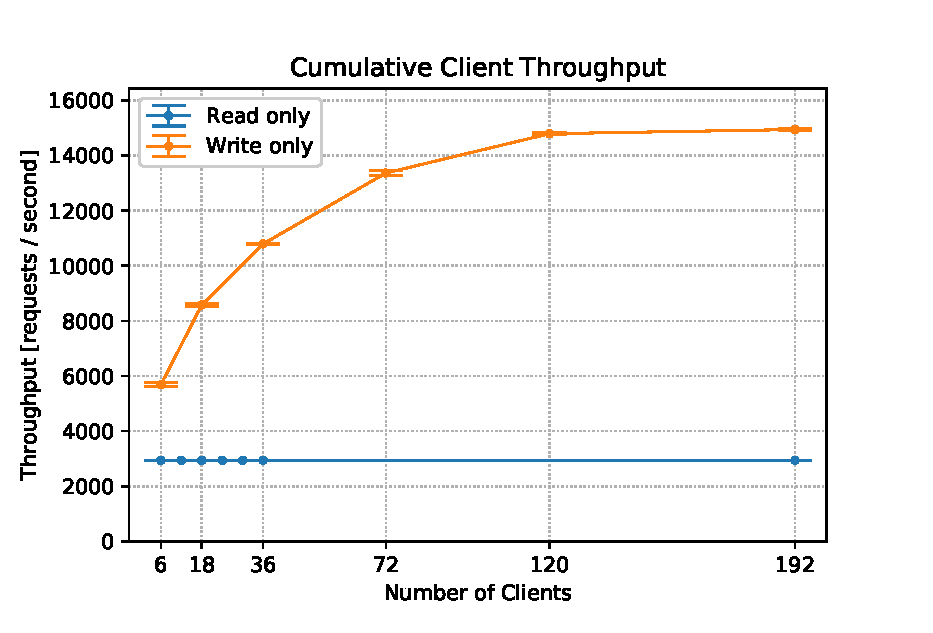
\includegraphics[width=1\linewidth]{plots/2_1_throughput.eps}
        \caption{Throughput}
    \end{subfigure}
    \begin{subfigure}{.5\textwidth}
        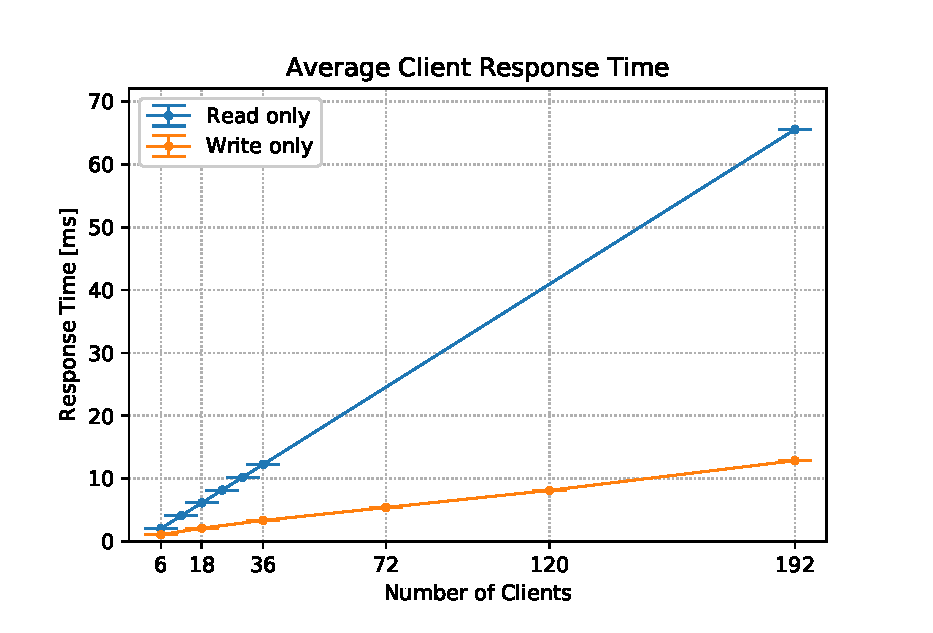
\includegraphics[width=1\linewidth]{plots/2_1_latency.eps}
        \caption{Response Time}
    \end{subfigure}
    \caption{Baseline without Middleware and one Server}
    \label{fig:2-1}
\end{figure}

\begin{table}
    \begin{center}
        \scriptsize{
          \begin{tabular}{|ccc|}
            \hline
            \textbf{Client} & \textbf{Middleware} & \textbf{Server}\\
            25.1 MB/s & 100.0 MB/s & 12.6 MB/s\\
            \hline
          \end{tabular}
        }
      \caption{Network Capacities (outgoing), measured using iperf}
      \label{link-caps}
    \end{center}
\end{table}

\subsubsection{Explanation}
%Describe in which phase the memcached servers are under-saturated, saturated, or over-saturated. Describe how throughput and response time correlate. Explain what further conclusions can be drawn from the experiment.
For read-only workload, the large value size of 4096 bytes causes GET responses to fully exhaust the outgoing capacity of the server's network link, while the CPU remains underutilized. Clearly, the bottleneck lies on the network capabilities, namely the upload, of the single memcached server. The collected dstat data shows an average upload of 12.41MB/s already for the first configuration with 6 virtual clients in total (see \autoref{dstat:2-1}). Because this value is very close to the maximum outgoing link capacity of the server machines shown in \autoref{link-caps}, which was measured using iperf, we can conclude that this indeed is the bottleneck in this system for read-only workload. The system is already with 6 virtual clients in total saturated because of the above mentioned bottleneck.

For write-only workload, the request size is large compared to the server response. The outgoing link capacity of the server should therefore not be the problem anymore. And indeed, this time outgoing network activities for both client and server machines stayed within their outgoing link capacities. However, for the memcached server a CPU utilization of 96\% has been measured for 32 virtual clients per thread as shown in \autoref{dstat:2-1} b). Clearly, the  bottleneck for the write-only workload is cpu bound on the memcached server side.
Up until 120 virtual clients in total the system  is under-saturated because with a higher amount of virtual clients the throughput increases until this point. After that point the system is in the saturation phase where the throughput stays the same while the response time increases linearly with more virtual clients.

The over-saturated phase has not been reached for both read and write-only during the experiments, this conclusion comes from the fact that only a linear increase of response time has been observed for an increasing amount of clients.

\begin{center}
    \begin{table}
    	\begin{tabular}{|l|p{2cm}|p{2cm}|p{2cm}|}
            \hline \textbf{Configuration} & \textbf{CPU} & \textbf{Send} & \textbf{Receive}\\
            \hline Server, read-only, 6 memtier clients in total & 11.0\%         & 12.41 MB/s    & 0.44 MB/s\\
            \hline Clients, read-only, 6 memtier clients in total & 5.44\%           & 0.16 MB/s     & 4.24 MB/s\\
            \hline Server, write-only,  120 memtier clients in total & 93.28\%        & 2.05 MB/s     & 63.33 MB/s\\
            \hline Clients, write-only, 120 memtier clients in total & 18.09\%       & 20.97 MB/s     & 0.69 MB/s\\
            \hline
    	\end{tabular}
	\caption{Machine Stats during Experiments for \autoref{sec2.1}}
    \label{dstat:2-1}
	\end{table}
\end{center}

\subsection{Two Servers} \label{sec2.2}
In this section, the maximum load generation capacity of a single memtier instance is examined. The measured throughput is presented as the total accumulated throughput of both memtier threads. The number of clients represents the total number of virtual clients across all three client machines. All results in this section are based on the output of memtier, which provides per second averages per virtual client. The first and last three seconds of each of the three repetitions were cut off as startup and cooldown time, leaving 60 seconds of data per repetition. All plots show averages and standard deviations across three repetitions of each configuration. The sanity of the data was checked with the interactive law for both throughput and response time separately and it was found that the interactive law aligns with the measured data. The configurations are shown in table \autoref{exp2-2} below.

\begin{table}
    \centering
	\begin{tabular}{|l|c|}
		\hline Number of servers                        & 2                        \\ 
		\hline Number of client machines                & 1                        \\ 
		\hline Instances of memtier per machine         & 2                        \\ 
		\hline Threads per memtier instance             & 1                        \\
		\hline Virtual clients per thread (write-only)  & [1,3,6,12,20,32]         \\ 
		\hline Virtual clients per thread (read-only)   & [1,2,3,4,5,6,32]         \\ 
		\hline Workload                                 & Write-only and Read-only \\
		\hline Repetitions                              & 
		3                        \\ 
		\hline 
	\end{tabular}
	\caption{Experiment configurations for \autoref{sec2.2}} \label{exp2-2}
\end{table}

\begin{figure}
    \begin{subfigure}{.5\textwidth}
        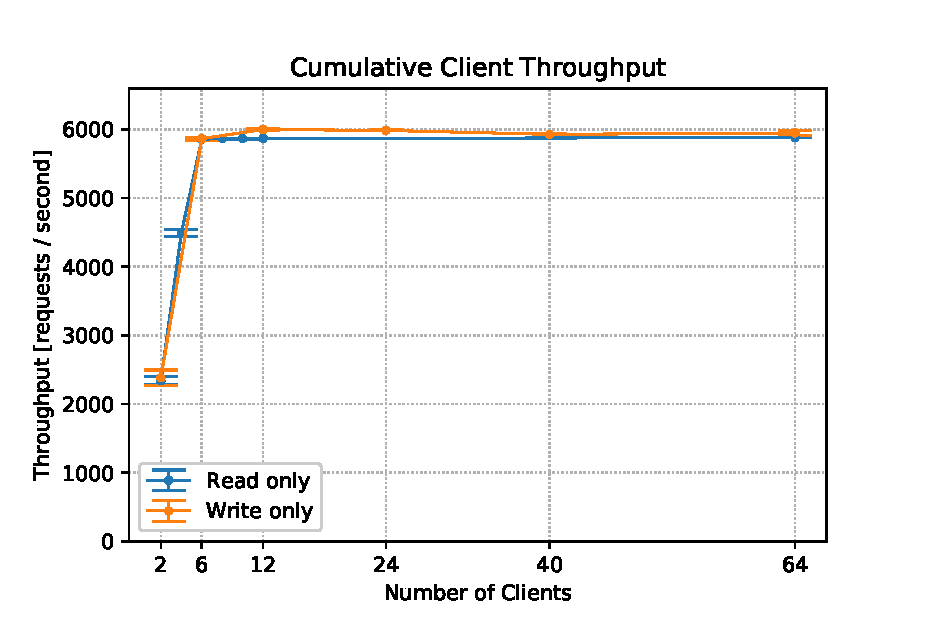
\includegraphics[width=1\linewidth]{plots/2_2_throughput.eps}
        \caption{Throughput}
    \end{subfigure}
    \begin{subfigure}{.5\textwidth}
        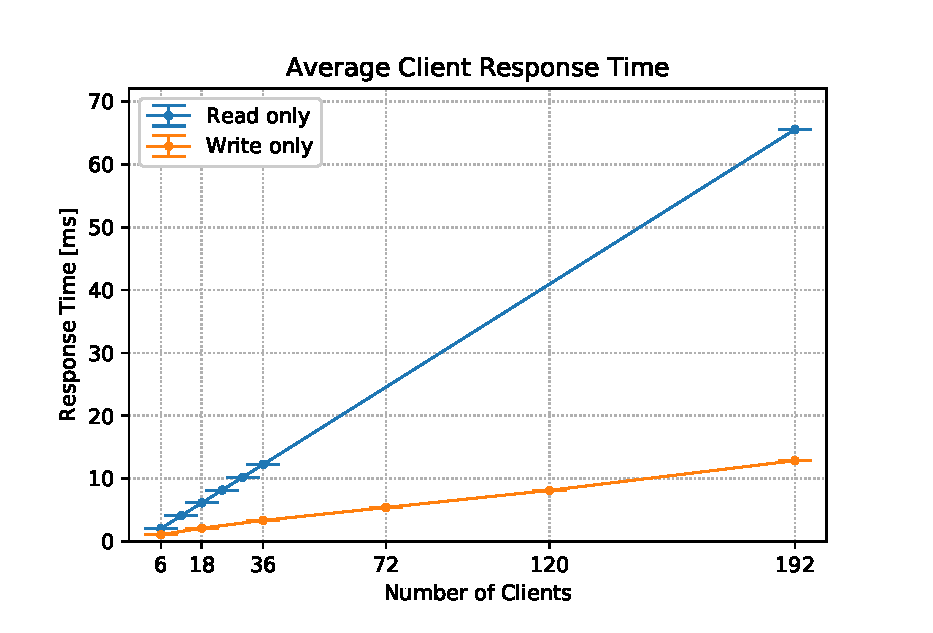
\includegraphics[width=1\linewidth]{plots/2_2_latency.eps}
        \caption{Response Time}
    \end{subfigure}
    \caption{Baseline without Middleware and two Servers}
    \label{fig:2-2}
\end{figure}
\subsubsection{Explanation}

%Describe how this experiment compares to the previous section. Which results are the same and which ones differ? Explain what further conclusions can be drawn from the experiment.

For read-only workload the system is under-saturated up until 8 virtual clients in total. This is derived from the fact that throughput is increasing significantly while the response time remains almost constant (see \autoref{fig:2-2}). From 8 virtual clients on, the throughput does not increase anymore while the response time continues to increase linearly. On the response time plot a knee is clearly visible. From this point on the system is saturated.
For read-only workload the bottleneck is again at the server, namely the outgoing network capacity. As can be seen in \autoref{dstat:2-2} (a) the server reaches an average outgoing network traffic of 12.47MB/s for 6 virtual memtier clients in total. This is very close to the previously presented maximum outgoing network capacity of the server machines (12.6MB/s) (see \autoref{link-caps}). Therefore, the system is saturated from 6 virtual memtier clients on. Before this point, the system is under-saturated for read-only workload.  An over-saturation has not been observed during the experiment. 

For write-only workload the system is under-saturated up until 6 virtual clients in total. This is derived from the fact that throughput is increasing significantly while the response time remains almost constant (see \autoref{fig:2-2}). From 6 virtual clients on, the throughput does not increase anymore while the response time continues to increase linearly. From this point on, the system is saturated.
For the write-only workload the bottleneck has been identified at the outgoing network capacity of the single memtier client. As shown in \autoref{dstat:2-2} (d) the client reaches an average outgoing network traffic of 24.80MB/s for 12 virtual memtier clients in total. This is very close to the maximum outgoing network capacity of the client machines (25.1MB/s) presented \autoref{link-caps}. Even though the increase of throughput is very little from 6 virtual clients to 12 virtual clients, the outgoing network traffic measured at the client machine for 6 virtual clients was 24.2MB/s which still is 0.9MB/s away from the measured maximum. This is the reason the beginning of the saturation phase starts only at 12 virtual clients for write-only workload and the maximum throughput is measured with 12 virtual clients. Before this point the system is under-saturated. An over-saturation has not been observed during the experiment.

\begin{center}
    \begin{table}
    	\begin{tabular}{|l|p{2cm}|p{2cm}|p{2cm}|}
            \hline \textbf{Configuration} & \textbf{CPU} & \textbf{Send} & \textbf{Receive}\\
            \hline Server, read-only, 8 memtier clients in total & 11.40\%         & 12.45 MB/s    & 0.44 MB/s\\
            \hline Clients, read-only, 8 memtier clients in total & 21.34\%           & 0.87 MB/s     & 24.95 MB/s\\
            \hline Server, write-only,  6 memtier clients in total & 12.50\%        & 0.42 MB/s     & 12.88 MB/s\\
            \hline Clients, write-only, 6 memtier clients in total & 17.91\%       & 24.66 MB/s     & 0.83 MB/s\\
            \hline
    	\end{tabular}
	\caption{Machine Stats during Experiments for \autoref{sec2.2}}
    \label{dstat:2-2}
	\end{table}
\end{center}



\subsection{Summary}

Based on the experiments above, fill out the following table:

\begin{center}
	{Maximum throughput of different VMs.}
	\begin{tabular}{|l|p{2cm}|p{2cm}|p{7cm}|}
		\hline                        & Read-only workload [req/s] & Write-only workload [req/s] & Configuration gives max. throughput \\ 
		\hline One memcached server   &          2937          &      14791               &            read-only: 6 virtual clients \newline write-only: 120 virtual clients                         \\ 
		\hline One load generating VM &        5847            &          5943           &         read-only: 8 virtual clients \newline write-only: 6 virtual clients                            \\ 
		\hline 
	\end{tabular}
\end{center}


\todo{Write at least two paragraphs about how both results relate. Describe what is the bottleneck of this setup is. If the maximum throughput for both experiments is the same, explain why. If it is not the case, explain why not. Write down key take-away messages about the behaviour of the memtier clients and the memcached servers.}

\section{Baseline with Middleware (90 pts)}

\subsection{One Middleware} \label{sec3.1}
After establishing baselines for memtier clients and memcached servers in \autoref{section2}, this section analyzes how adding my middleware to the system affects the preformance. Due to the additional network hops from client to middleware and from middleware to server it is unavoidable that some additional latency is introduced. The middleware is designed to hide this latency with parallelism using its worker threads and, given a sufficient amount of parallelism, avoid becoming the system's bottleneck.

The results in this section are based on the aggregated request logs from the middleware. The first and last three seconds of each of the three repetitions were cut off as startup and cooldown time, leaving 60 seconds of data per repetition. As a sanity check, the same data has been extracted from the aggregated memtier client outputs, compared and found to align well. No misses occurred during the test and all client requests were processed and answered. As before, the number of clients represents the total number of virtual clients across all three client machines. All plots show averages and standard deviations across three repetitions of each configuration. The sanity of the data has been checked with the interactive law for both throughput and response time separately for all configurations and it was found that the interactive law aligns with the measured data. The configurations examined for this section are shown in \autoref{exp3-1} below.



\begin{table}
    \centering
	\begin{tabular}{|l|c|}
		\hline Number of servers                & 1                        \\ 
		\hline Number of client machines        & 3                        \\ 
		\hline Instances of memtier per machine & 1                        \\ 
		\hline Threads per memtier instance     & 2                        \\
		\hline Virtual clients per thread (write-only)  & [1,3,6,12,20,32] \\ 
		\hline Virtual clients per thread (read-only)   & [1,2,3,4,5,6,32] \\ 
		\hline Workload                         & Write-only and Read-only \\
		\hline Number of middlewares            & 1                        \\
		\hline Worker threads per middleware    & [8, 16, 32, 64]          \\
		\hline Repetitions                      & 3                        \\ 
		\hline 
	\end{tabular}
	\caption{Experiment configurations for Section 3.1} \label{exp3-1}
\end{table}

\begin{figure}
    \begin{subfigure}{.5\textwidth}
        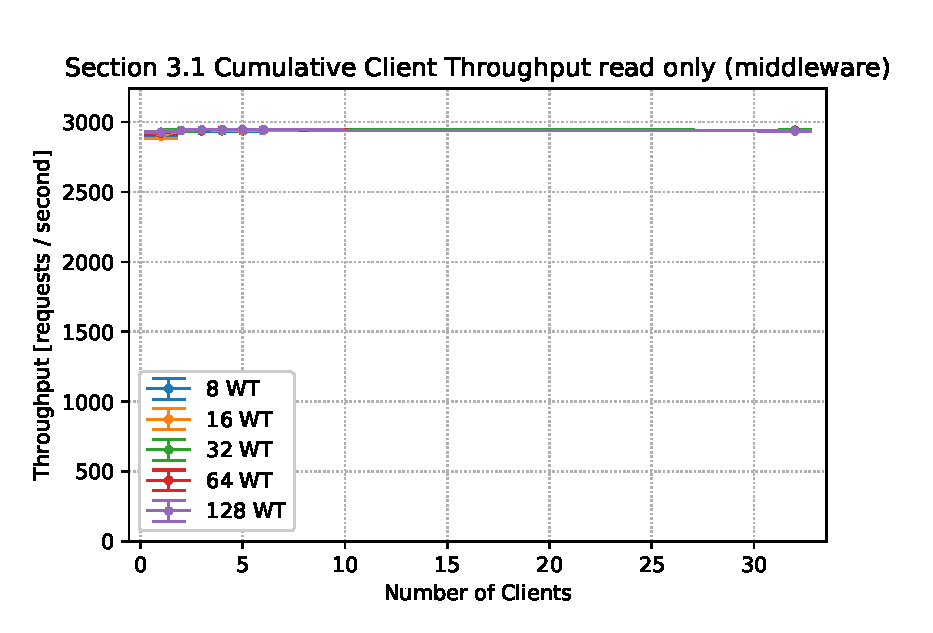
\includegraphics[width=1\linewidth]{plots/3_1a_throughputMiddleware.eps}
        \caption{Throughput, read only}
    \end{subfigure}
    \begin{subfigure}{.5\textwidth}
        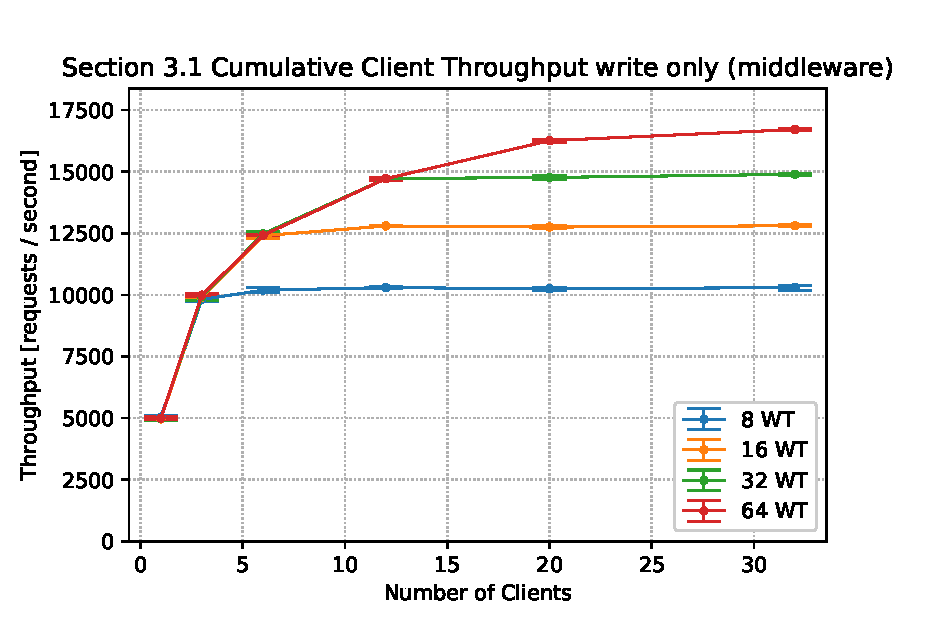
\includegraphics[width=1\linewidth]{plots/3_1b_throughputMiddleware.eps}
        \caption{Throughput, write only}
    \end{subfigure}
    \caption{Throughput of baseline with one Middleware, one Server, \autoref{sec3.1}}
    \label{fig:3-1-throughput}
\end{figure}

\begin{figure}
    \begin{subfigure}{.5\textwidth}
        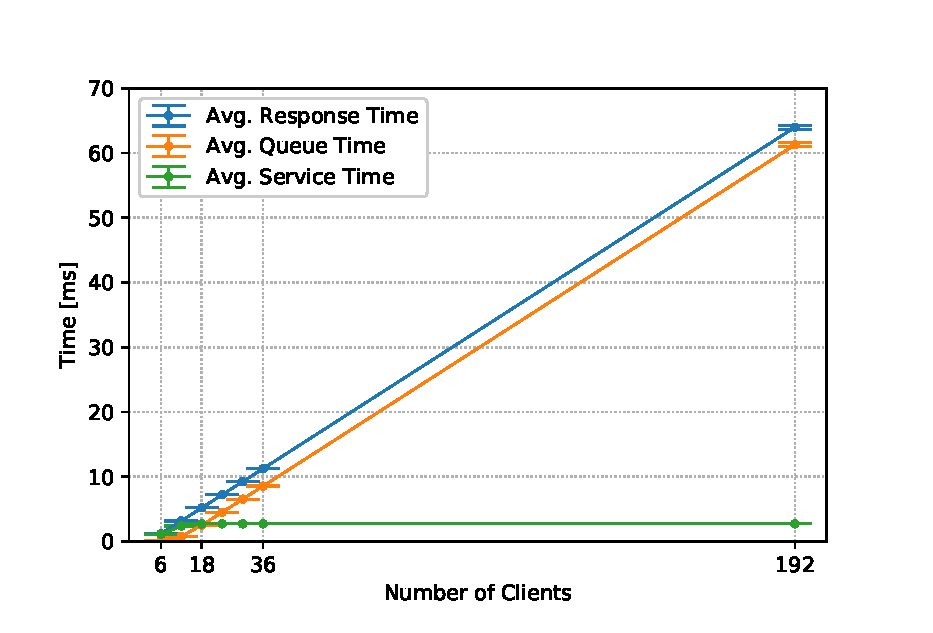
\includegraphics[width=1\linewidth]{plots/3_1a_extendedLatencyMiddleware_8w.eps}
        \caption{8 worker threads}
    \end{subfigure}
    \begin{subfigure}{.5\textwidth}
        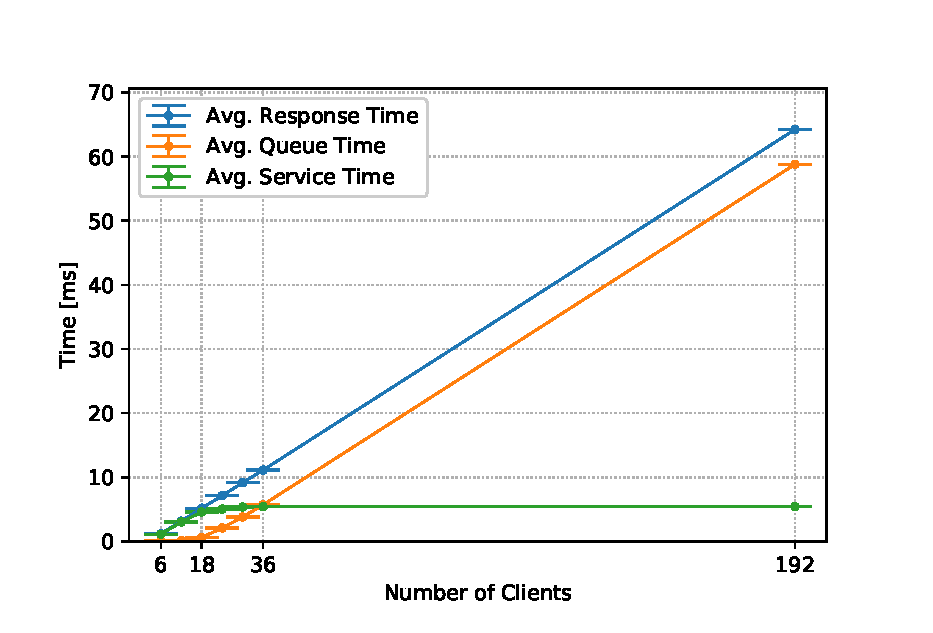
\includegraphics[width=1\linewidth]{plots/3_1a_extendedLatencyMiddleware_16w.eps}
        \caption{16 worker threads}
    \end{subfigure}
    \begin{subfigure}{.5\textwidth}
        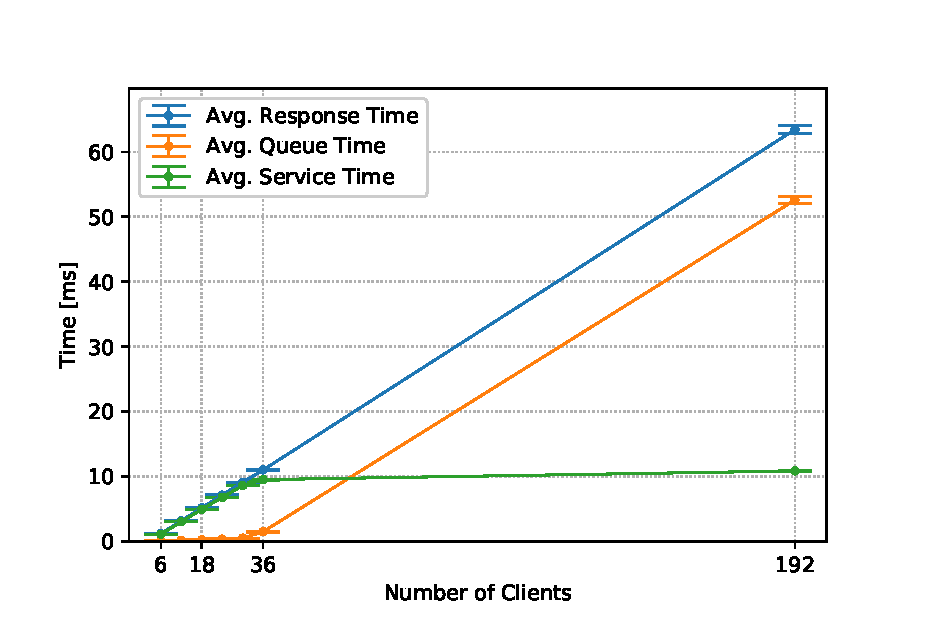
\includegraphics[width=1\linewidth]{plots/3_1a_extendedLatencyMiddleware_32w.eps}
        \caption{32 worker threads}
    \end{subfigure}
    \begin{subfigure}{.5\textwidth}
        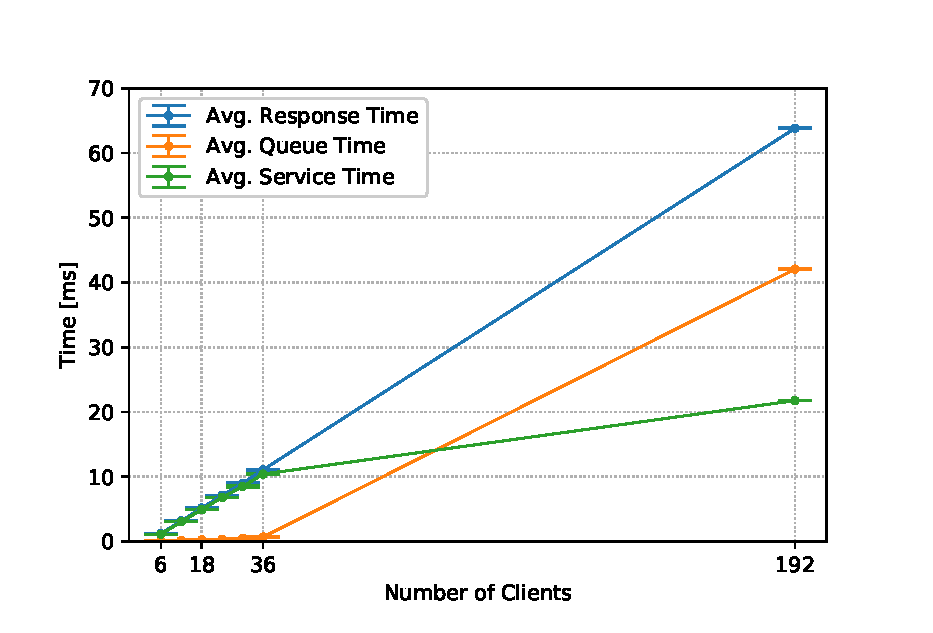
\includegraphics[width=1\linewidth]{plots/3_1a_extendedLatencyMiddleware_64w.eps}
        \caption{64 worker threads}
    \end{subfigure}

    \caption{Response-, Queue- and Server-Service-Times of baseline with one Middleware, one Server, \autoref{sec3.1}, Read-only workload}
    \label{fig:3-1-times-readonly}
\end{figure}

\begin{figure}
    \begin{subfigure}{.5\textwidth}
        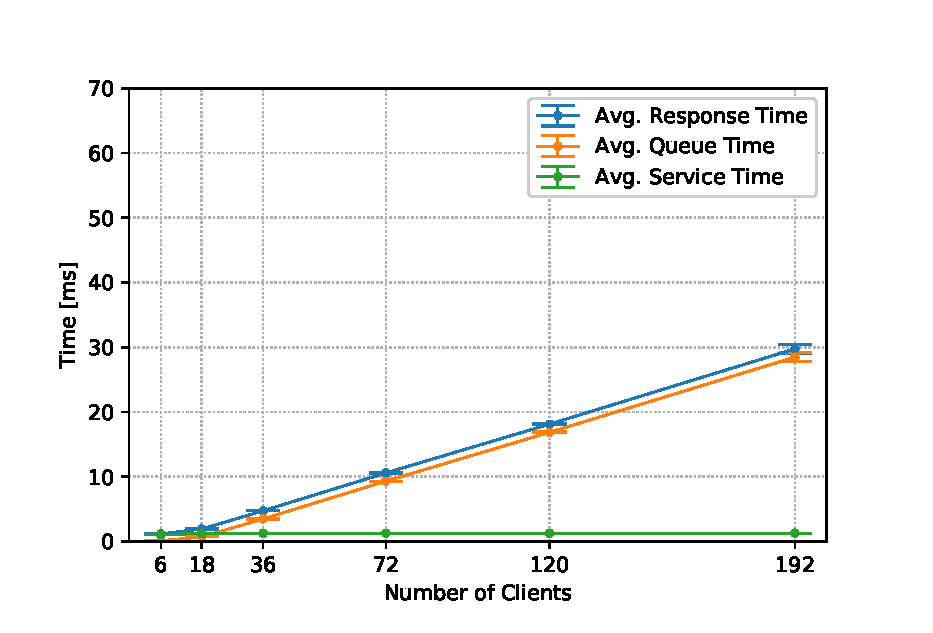
\includegraphics[width=1\linewidth]{plots/3_1b_extendedLatencyMiddleware_8w.eps}
        \caption{8 worker threads}
    \end{subfigure}
    \begin{subfigure}{.5\textwidth}
        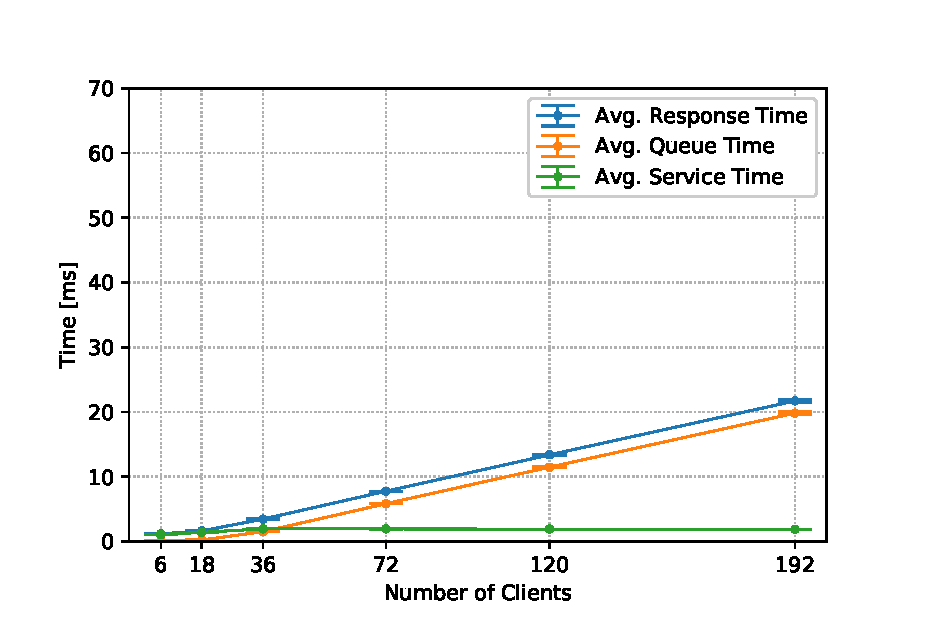
\includegraphics[width=1\linewidth]{plots/3_1b_extendedLatencyMiddleware_16w.eps}
        \caption{16 worker threads}
    \end{subfigure}
    \begin{subfigure}{.5\textwidth}
        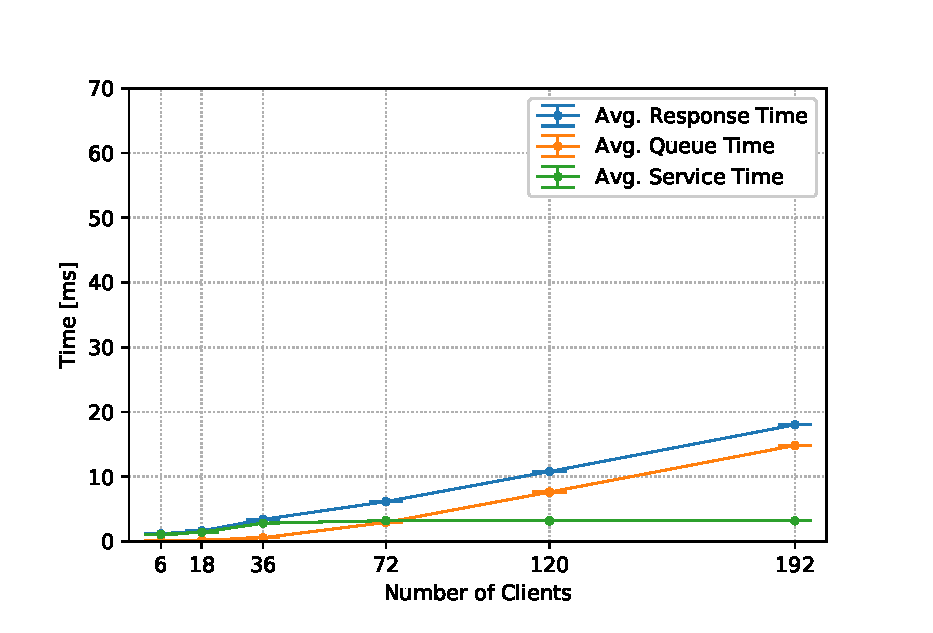
\includegraphics[width=1\linewidth]{plots/3_1b_extendedLatencyMiddleware_32w.eps}
        \caption{32 worker threads}
    \end{subfigure}
    \begin{subfigure}{.5\textwidth}
        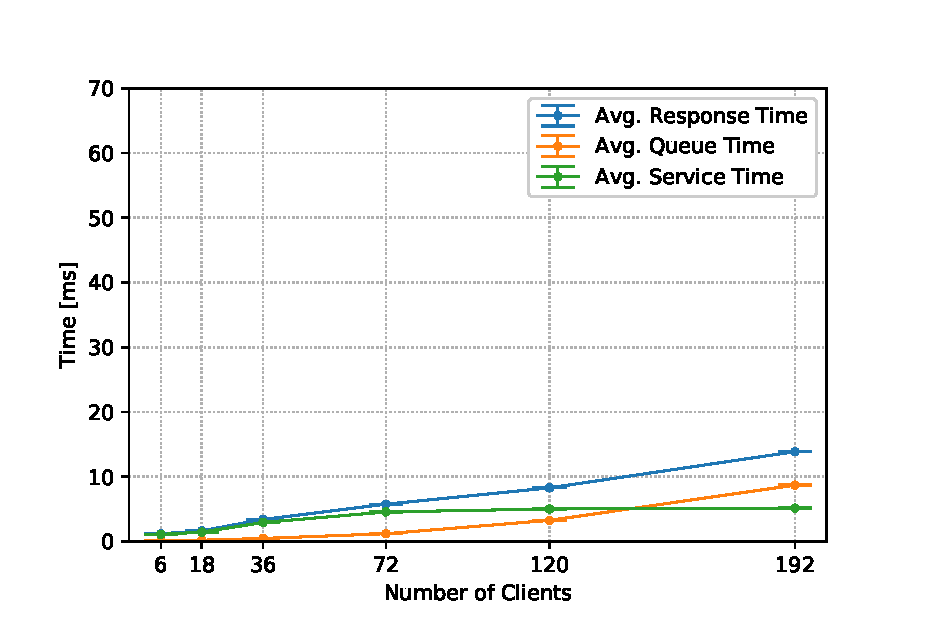
\includegraphics[width=1\linewidth]{plots/3_1b_extendedLatencyMiddleware_64w.eps}
        \caption{64 worker threads}
    \end{subfigure}

    \caption{Response-, Queue- and Server-Service-Times of baseline with one Middleware, one Server, \autoref{sec3.1}, Write-only workload}
    \label{fig:3-1-times-writeonly}
\end{figure}

\begin{center}
    \begin{table}
    	\begin{tabular}{|l|p{2cm}|p{2cm}|p{2cm}|}
            \hline \textbf{Configuration} & \textbf{CPU} & \textbf{Send} & \textbf{Receive}\\
            \hline Server, read-only, 8WT, 6 memtier clients in total & 10.75\%         & 12.20 MB/s    & 0.43 MB/s\\
            \hline Server, read-only, 16WT, 6 memtier clients in total & 11.35\%         & 12.17 MB/s    & 0.43 MB/s\\
            \hline Server, read-only, 32WT, 6 memtier clients in total & 13.62\%         & 12.27 MB/s    & 0.43 MB/s\\
            \hline Server, read-only, 64WT, 6 memtier clients in total & 15.01\%         & 12.24 MB/s    & 0.43 MB/s\\
            \hline
    	\end{tabular}
	\caption{Machine Stats during read-only Experiments for \autoref{sec3.1}}
    \label{dstat:3-1}
	\end{table}
\end{center}


\begin{center}
    \begin{table}
    	\begin{tabular}{|l|p{2cm}|p{2cm}|p{2cm}|}
            \hline \textbf{Configuration} & \textbf{CPU} & \textbf{Send} & \textbf{Receive}\\
            \hline Server, write-only, 8WT, 192 memtier clients in total & 21.96\%         & 0.86 MB/s    & 26.51 MB/s\\
            \hline Server, write-only, 16WT, 192 memtier clients in total & 45.52\%         & 1.17 MB/s    & 36.14 MB/s\\
            \hline Server, write-only, 32WT, 192 memtier clients in total & 65.48\%         & 1.39 MB/s    & 42.81 MB/s\\
            \hline Server, write-only, 64WT, 192 memtier clients in total & 80.70\%         & 1.71 MB/s    & 52.65 MB/s\\
            \hline Server, write-only, 128WT, 192 memtier clients in total & 90.87\%         & 1.94 MB/s    & 59.75 MB/s\\
            \hline
    	\end{tabular}
	\caption{Machine Stats during write-onlyExperiments for \autoref{sec3.1}}
    \label{dstat:3-1wo}
	\end{table}
\end{center}

\subsubsection{Explanation}

% Provide a detailed analysis of the results (e.g., bottleneck analysis, component utilizations, average queue lengths, system saturation). Add any additional figures and experiments that help you illustrate your point and support your claims.
For read-only workload the server reaches its maximum outgoing network capacity of 12.5MB/s already almost with 6 memtier clients in total. As \autoref{dstat:3-1} shows, the measured send capacity of dstat shows for all worker thread configurations a maximum of around 12.2MB/s. With 12 memtier clients in total this value increases up to 12.4MB/s in average. Because this corresponds to an increase of only 40 requests per second the entering of saturation phase is chosen to be at 6 memtier clients in total. From this point on, the system is in saturation phase as can be seen on \autoref{fig:3-1-throughput} (a) for all configurations of worker threads. Hence, no under- and no over-saturation phase has been observed for read-only workload.
A maximum throughput of 2939 requests per second is reached, which is equivalent to the maximum throughput for read-only workload measured in \autoref{sec2.1}.
Like in \autoref{sec2.1} bottleneck is the single memcached server with its limited outgoing network capacity.
\autoref{fig:3-1-times-readonly} shows how the average service time, the time the server needs to respond to a request from the middleware, increases with more worker threads. This comes from the fact that more connections to the single memcached server are established in parallel. The figure also shows nicely how the queuing time in the middleware remains almost zero up until the number of memtier clients exceeds the number of worker threads. Up until the point where there are at least as many worker threads as clients connecting, because we are in a closed system and clients send requests only one after another, each request is taken from the queue immediately.


For write-only workload the situation is different. This time the server is not the bottleneck up until 64 worker threads. \autoref{fig:3-1-throughput} (b) shows nicely how the throughput increases with more worker threads. This leads to the conclusion that the middleware is the bottleneck, because if the number of worker threads in the middleware is increased, the throughput increases too. The dstat logs of all machines confirm this hypothesis and show that the network traffic stays within the maximum capacities listed in \autoref{link-caps} and the CPU usage of all machines stays below 70\%.
\autoref{dstat:3-1wo} shows tif the number of worker threads is further increased to 128, the CPU usage of the server rises up until 90\% which is an indicator that the server is now the bottleneck and more worker threads will not lead to a higher throughput from this point on.
For 8 and 16 worker threads the system is under-saturated until 18 clients, as the average response time remains constant up until this point as shown in \autoref{fig:3-1-times-writeonly} (a) and (b) and then starts to increase linearly.
For 32 worker threads the system is under-saturated unitl 36 clients, again, the average response time remains constant up until this point and then starts to increase linearly as shown in \autoref{fig:3-1-times-writeonly} (c).
For 64 worker threads the system changes from under-saturated to saturated at 72 clients, as the average response time remains almost constant up until this point as shown in \autoref{fig:3-1-times-writeonly} (d) and then increases linearly.
From this observation we conclude that the middleware is under-saturated until the number of clients is at least as large as the number of worker threads. From then on the queue in the middleware is not empty anymore and saturation phase is reached.
No over-saturation has been observed during this experiment.
\todo{explain why response time is much lower compared to read-only workload.}



\subsection{Two Middlewares} \label{sec3.2}

In this section the preformance of two middlewares is investigated, splitting the load into two, connecting each client machine to both middlewares.

The results in this section are based on the aggregated request logs from the two middlewares. The first and last three seconds of each of the three repetitions were cut off as startup and cooldown time, leaving 60 seconds of data per repetition. As a sanity check, the same data has been extracted from the aggregated memtier client outputs, compared and found to align well. No misses occurred during the test and all client requests were processed and answered. As before, the number of clients represents the total number of virtual clients across all three client machines. All plots show averages and standard deviations across three repetitions of each configuration. The sanity of the data has been checked with the interactive law for both throughput and response time separately for all configurations and it was found that the interactive law aligns with the measured data. The configurations examined for this section are shown in \autoref{exp3-2} below.

\begin{table}
    \centering
	\begin{tabular}{|l|c|}
		\hline Number of servers                & 1                        \\ 
		\hline Number of client machines        & 3                        \\ 
		\hline Instances of memtier per machine & 2                        \\ 
		\hline Threads per memtier instance     & 1                        \\
		\hline Virtual clients per thread (write-only)  & [1,3,6,12,20,32] \\ 
		\hline Virtual clients per thread (read-only)   & [1,2,3,4,5,6,32] \\ 
		\hline Workload                         & Write-only and Read-only \\
		\hline Number of middlewares            & 2                        \\
		\hline Worker threads per middleware    & [8, 16, 32, 64]          \\
		\hline Repetitions                      & 3                        \\ 
		\hline 
	\end{tabular}
	\caption{Experiment configurations for \autoref{sec3.2}} \label{exp3-2}
\end{table}

\begin{figure}
    \begin{subfigure}{.5\textwidth}
        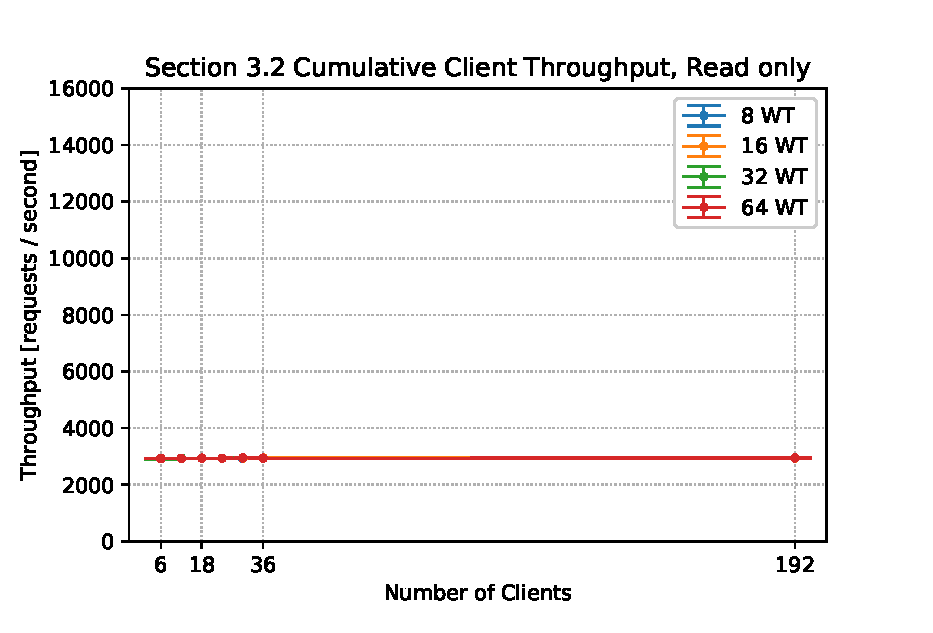
\includegraphics[width=1\linewidth]{plots/3_2a_throughputMiddleware.eps}
        \caption{Throughput, read only}
    \end{subfigure}
    \begin{subfigure}{.5\textwidth}
        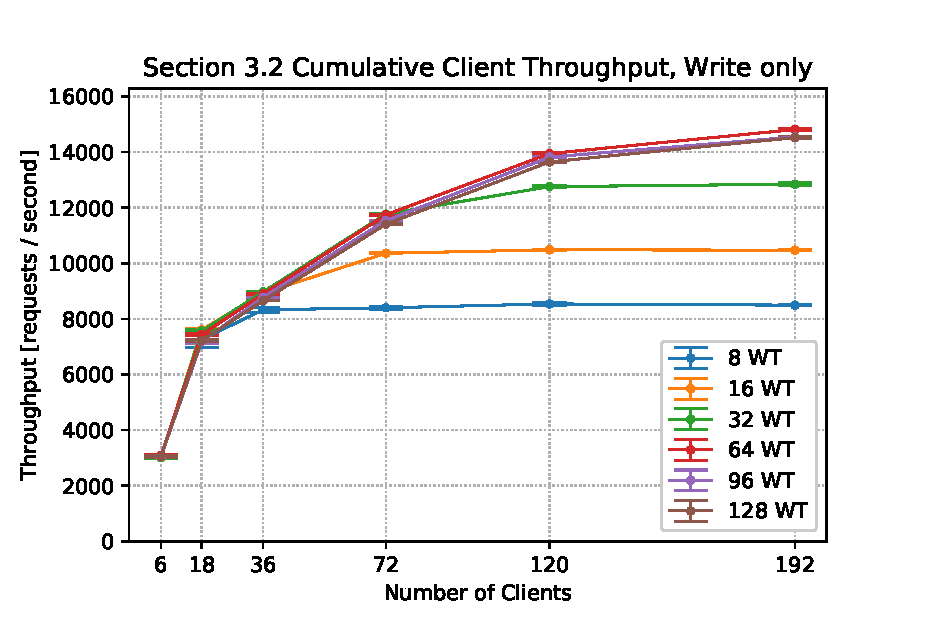
\includegraphics[width=1\linewidth]{plots/3_2b_throughputMiddleware.eps}
        \caption{Throughput, write only}
    \end{subfigure}

    \caption{Throughput of baseline with two Middlewares, one Server, \autoref{sec3.2}}
    \label{fig:3-2-throughput}
\end{figure}


\begin{figure}
    \begin{subfigure}{.5\textwidth}
        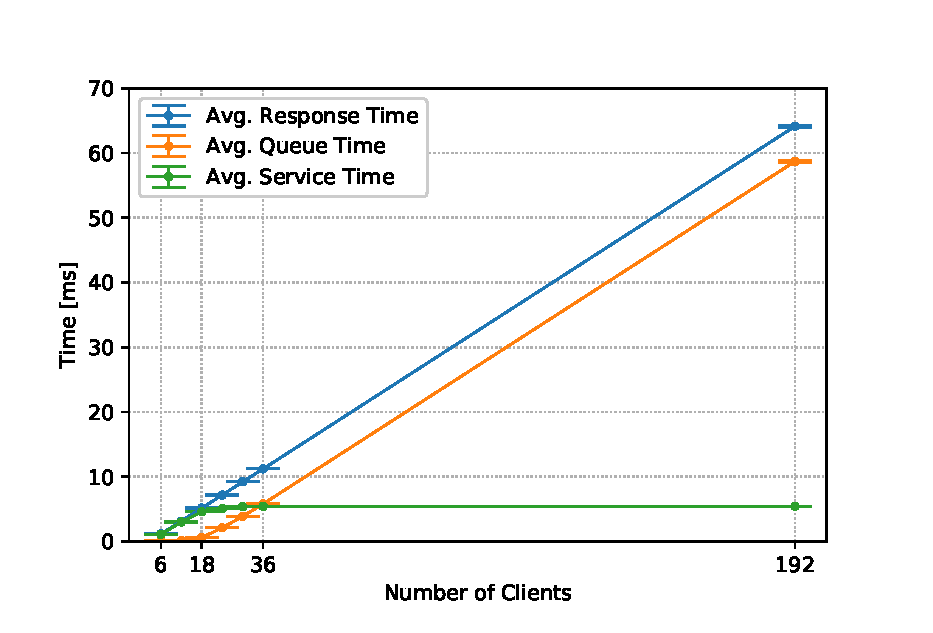
\includegraphics[width=1\linewidth]{plots/3_2a_extendedLatencyMiddleware_8w.eps}
        \caption{8 worker threads}
    \end{subfigure}
    \begin{subfigure}{.5\textwidth}
        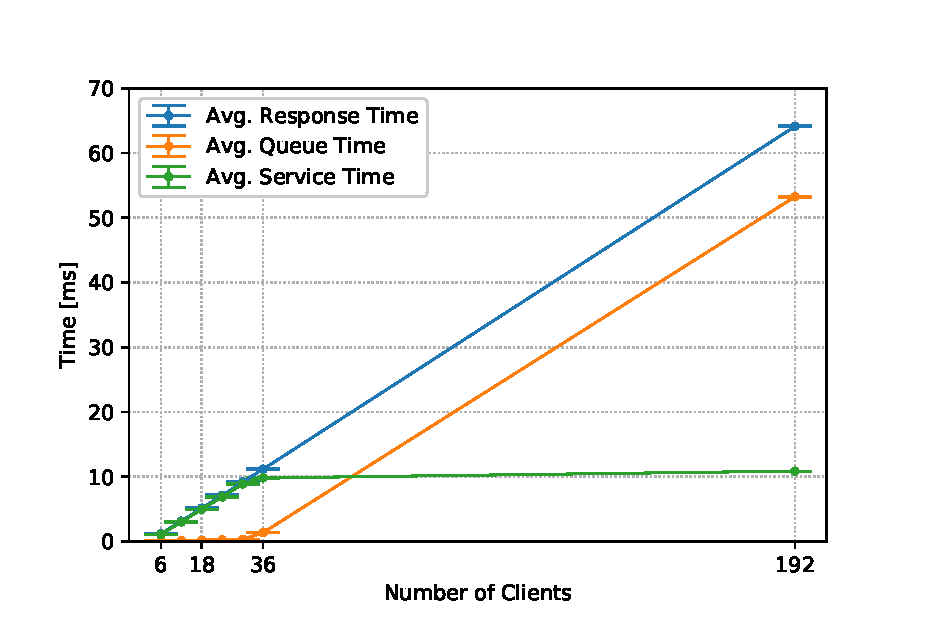
\includegraphics[width=1\linewidth]{plots/3_2a_extendedLatencyMiddleware_16w.eps}
        \caption{16 worker threads}
    \end{subfigure}
    \begin{subfigure}{.5\textwidth}
        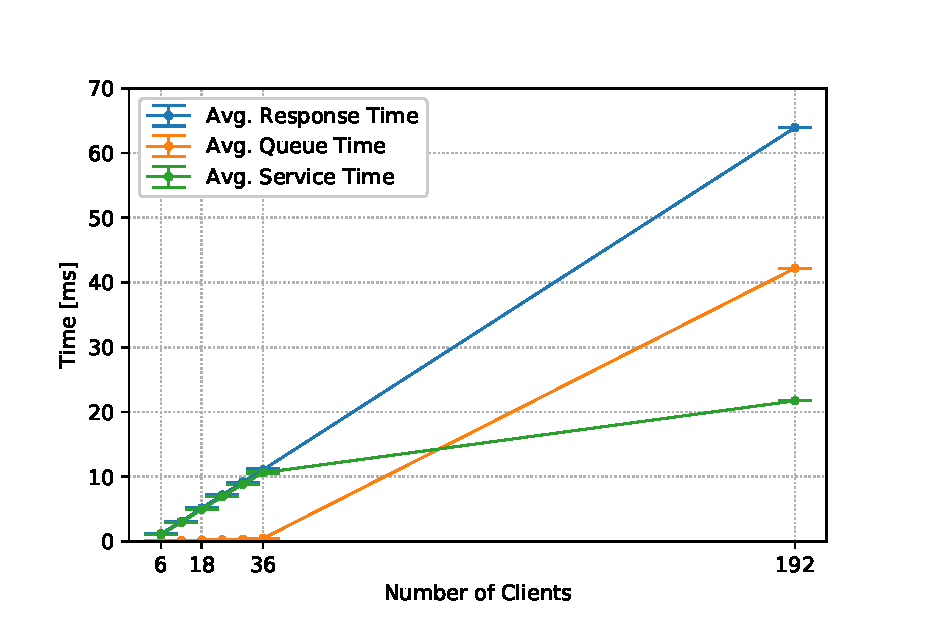
\includegraphics[width=1\linewidth]{plots/3_2a_extendedLatencyMiddleware_32w.eps}
        \caption{32 worker threads}
    \end{subfigure}
    \begin{subfigure}{.5\textwidth}
        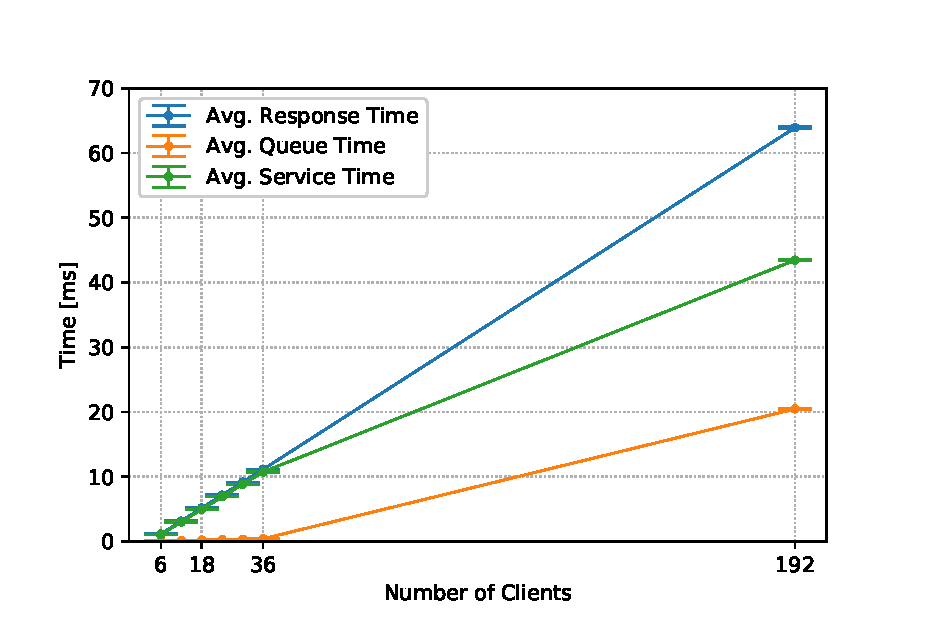
\includegraphics[width=1\linewidth]{plots/3_2a_extendedLatencyMiddleware_64w.eps}
        \caption{64 worker threads}
    \end{subfigure}

    \caption{Response-, Queue- and Server-Service-Times of baseline with two Middlewares, one Server, \autoref{sec3.2}, Read-Only workload}
    \label{fig:3-2-times-readonly}
\end{figure}

\begin{figure}
    \begin{subfigure}{.5\textwidth}
        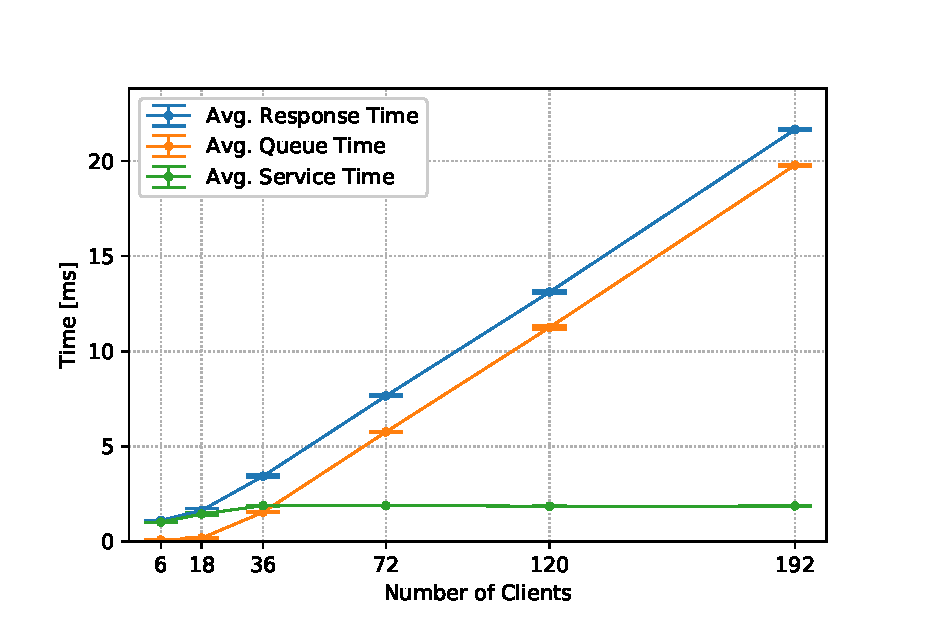
\includegraphics[width=1\linewidth]{plots/3_2b_extendedLatencyMiddleware_8w.eps}
        \caption{8 worker threads}
    \end{subfigure}
    \begin{subfigure}{.5\textwidth}
        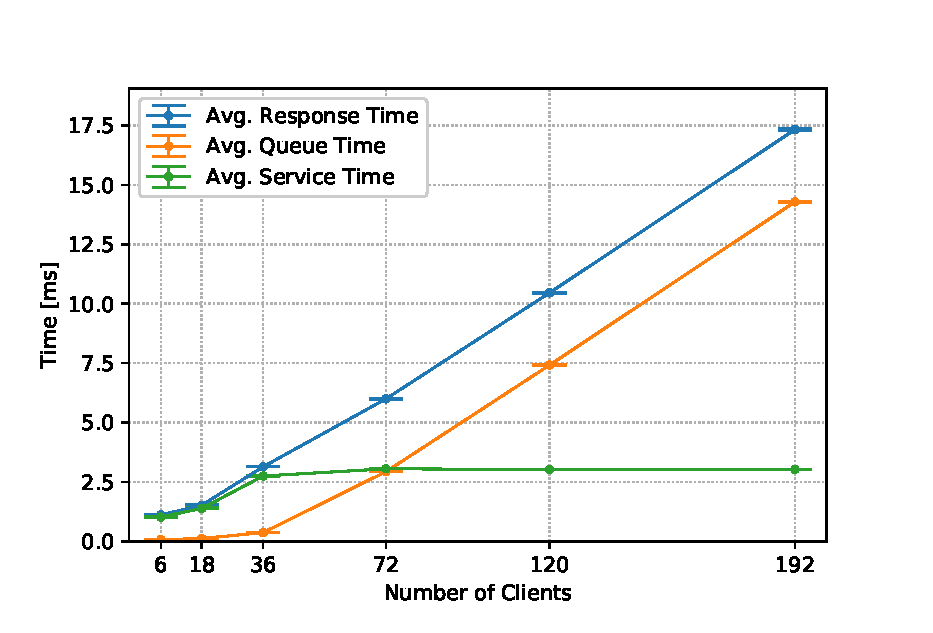
\includegraphics[width=1\linewidth]{plots/3_2b_extendedLatencyMiddleware_16w.eps}
        \caption{16 worker threads}
    \end{subfigure}
    \begin{subfigure}{.5\textwidth}
        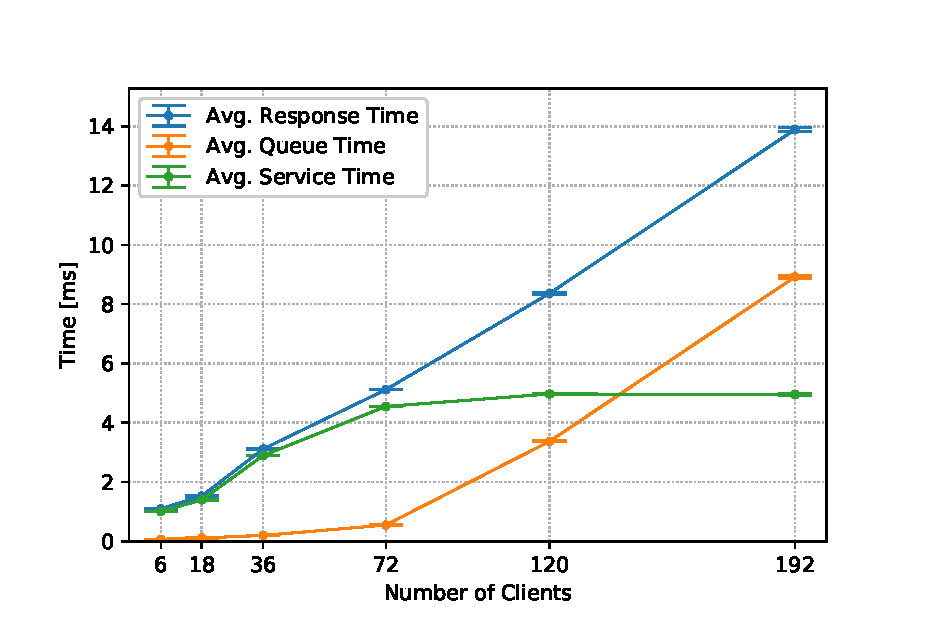
\includegraphics[width=1\linewidth]{plots/3_2b_extendedLatencyMiddleware_32w.eps}
        \caption{32 worker threads}
    \end{subfigure}
    \begin{subfigure}{.5\textwidth}
        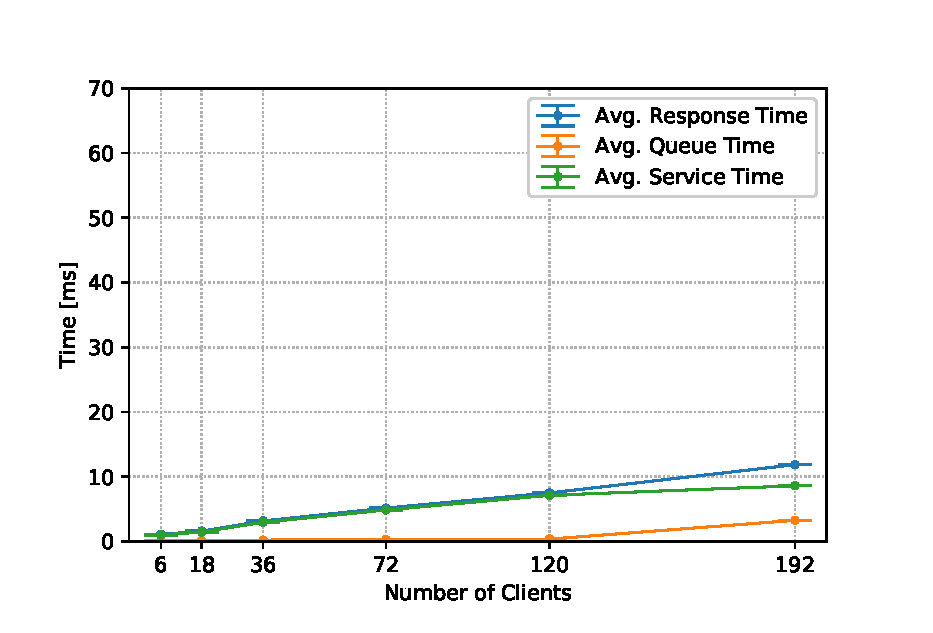
\includegraphics[width=1\linewidth]{plots/3_2b_extendedLatencyMiddleware_64w.eps}
        \caption{64 worker threads}
    \end{subfigure}

    \caption{Response-, Queue- and Server-Service-Times of baseline with two Middlewares, one Server, \autoref{sec3.2}, Write-Only workload}
    \label{fig:3-2-times-writeonly}
\end{figure}

\begin{center}
    \begin{table}
    	\begin{tabular}{|l|p{2cm}|p{2cm}|p{2cm}|}
            \hline \textbf{Configuration} & \textbf{CPU} & \textbf{Send} & \textbf{Receive}\\
            \hline Server, read-only, 8WT, 6 memtier clients in total & 11.73\%         & 12.29 MB/s    & 0.43 MB/s\\
            \hline Server, read-only, 16WT, 6 memtier clients in total & 14.25 \%         & 12.29MB/s    & 0.43 MB/s\\
            \hline Server, read-only, 32WT, 6 memtier clients in total & 14.97\%         & 12.25 MB/s    & 0.43 MB/s\\
            \hline Server, read-only, 64WT, 6 memtier clients in total & 16.14\%         & 12.26 MB/s    & 0.43 MB/s\\
            \hline
    	\end{tabular}
	\caption{Machine Stats during read-only Experiments for \autoref{sec3.2}, two middlewares}
    \label{dstat:3-2}
	\end{table}
\end{center}

\begin{center}
    \begin{table}
    	\begin{tabular}{|l|p{2cm}|p{2cm}|p{2cm}|}
            \hline \textbf{Configuration} & \textbf{CPU} & \textbf{Send} & \textbf{Receive}\\
            \hline Server, write-only, 8WT, 192 memtier clients in total & 51.19\%         & 1.18 MB/s    & 36.37 MB/s\\
            \hline Server, write-only, 16WT, 192 memtier clients in total & 65.11\%         & 1.45 MB/s    & 44.75 MB/s\\
            \hline Server, write-only, 32WT, 192 memtier clients in total & 81.20\%         & 1.77 MB/s    & 54.75 MB/s\\
            \hline Server, write-only, 64WT, 192 memtier clients in total & 93.17\%         & 2.05 MB/s    & 63.48 MB/s\\
            \hline Server, write-only, 128WT, 192 memtier clients in total & 95.18\%         & 2.02 MB/s    & 62.38 MB/s\\
            \hline
    	\end{tabular}
	\caption{Machine Stats during write-only Experiments for \autoref{sec3.2}, two middlewares}
    \label{dstat:3-2wo}
	\end{table}
\end{center}


\subsubsection{Explanation}
For read-only workload we observe the exact same throughput as in \autoref{sec3.1} for read-only workload. This is no surprise as also with two middlewares the server network upload reaches its maximum upload capacity already with 6 memtier clients. \autoref{dstat:3-2} shows several machine stats measured with dstat during the experiments for several worker thread configurations.
The tresponse, queue and service times plotted in \autoref{fig:3-2-times-readonly} look very similar as in \autoref{sec3.1} but is shifted by one graph because 8 worker threads is now equal to the 16 worker threads graph of \autoref{sec3.1}, the 16 worker threads graph is equal to the 32 worker threads graph and so on. This is the case because doubling the amount of middlewares is equal to doubling the amount of worker threads (despite some overhead of the second middleware instance).

For write-only workload we also observe a similar throughput as in \autoref{sec3.1}, with the maximum throughput of 8 worker threads being equal to 16 worker threads in \autoref{sec3.1}. \autoref{fig:3-2-throughput} shows again that the two middlewares are the bottleneck up until 32 worker threads because an increase of worker threads leads to an increase of throughput. For 64 worker threads \autoref{dstat:3-2wo} shows a CPU usage of over 93\% on the server which implies that the bottleneck now lies at the server and that a further increase of worker thread would not lead to an increase in throughput.
Furthermore, \autoref{fig:3-2-throughput} shows that doubling the number of middleware is almost equal to doubling the amount of workerthreads.
\todo{explain why throughput is slightly higher for 2x middleware compared to 2x workerthreads?!}


\subsection{Summary}

%Based on the experiments above, fill out the following table. For both of them use the numbers from a single experiment to fill out all lines. Miss rate represents the percentage of GET requests that return no data. Time in the queue refers to the time spent in the queue between the net-thread and the worker threads.
\todo{write summary, comment throughput/response time table below}


\begin{center}
	{Maximum throughput for one middleware.}
	\begin{tabular}{|l|p{2cm}|p{2cm}|p{2cm}|p{2cm}|}
		\hline                                                   & Throughput [req/s]    & Response time & Average time in queue & Miss rate \\ 
		\hline Reads: Measured on middleware (8WT, 12 clients)   &     2939       &    3.15ms     & 0.79ms                & 0.0       \\ 
		\hline Reads: Measured on clients (8WT, 12 clients)      &     2939       &    4.1ms      & n/a                   & 0.0       \\ 
		\hline Writes: Measured on middleware (64WT, 120 clients)&     12030      &    8.27ms     & 3.24ms                & n/a       \\ 
		\hline Writes: Measured on clients (64WT, 120 clients)   &     12034      &    9.97ms     & n/a                   & n/a       \\ 
		\hline 
	\end{tabular}
\end{center}

\begin{center}
	{Maximum throughput for two middlewares.}
	\begin{tabular}{|l|p{2cm}|p{2cm}|p{2cm}|p{2cm}|}
		\hline                                                    & Throughput [req/s]    & Response time & Average time in queue & Miss rate \\ 
		\hline Reads: Measured on middleware (8WT, 12 clients)    &    2935        &   3.12ms      &   0.12ms              & 0.0       \\ 
		\hline Reads: Measured on clients(8WT, 12 clients)        &    2935        &   4.08ms      & n/a                   & 0.0       \\ 
		\hline Writes: Measured on middleware (64WT, 192 clients) &    14810       &   11.84ms     &   3.25ms              & n/a       \\ 
		\hline Writes: Measured on clients (64WT, 192 clients)    &    14813       &   12.96ms     & n/a                   & n/a       \\ 
		\hline 
	\end{tabular}
\end{center}

Based on the data provided in these tables, write at least two paragraphs summarizing your findings about the performance of the middleware in the baseline experiments.

\section{Throughput for Writes (90 pts)}

\subsection{Full System} \label{sec4}
The setup from the previous section is now expanded even further for write-only workload. In this experiment the effect of replication can be observed as each middleware is replicating the SET requests to all three memcached servers.

The results in this section are based on the aggregated request logs from the two middlewares. The first and last three seconds of each of the three repetitions were cut off as startup and cooldown time, leaving 60 seconds of data per repetition. As a sanity check, the same data has been extracted from the aggregated memtier client outputs, compared and found to align well. No misses occurred during the test and all client requests were processed and answered. As before, the number of clients represents the total number of virtual clients across all three client machines. All plots show averages and standard deviations across three repetitions of each configuration. The sanity of the data has been checked with the interactive law for both throughput and response time separately for all configurations and it was found that the interactive law aligns with the measured data. The configurations examined for this section are shown in \autoref{exp4} below.
%Connect three load generating VMs to two middlewares and three memchached servers. Run a write-only experiment. 
%You need to plot throughput and response time measured on the middleware as a function of number of clients. The measurements have to be performed for 8, 16, 32 and 64 worker threads inside each middleware.

\begin{table}
    \centering
	\begin{tabular}{|l|c|}
		\hline Number of servers                & 3                         \\ 
		\hline Number of client machines        & 3                         \\ 
		\hline Instances of memtier per machine & 2                         \\ 
		\hline Threads per memtier instance     & 1                         \\
		\hline Virtual clients per thread       & [1, 3, 6, 12, 20, 32]     \\ 
		\hline Workload                         & Write-only                \\
		\hline Number of middlewares            & 2                         \\
		\hline Worker threads per middleware    & [8, 16, 32, 64]           \\
		\hline Repetitions                      & 3                         \\ 
		\hline 
	\end{tabular}
	\caption{Experiment configurations for \autoref{sec4}} \label{exp4}
\end{table}

\begin{figure}
    \centering
    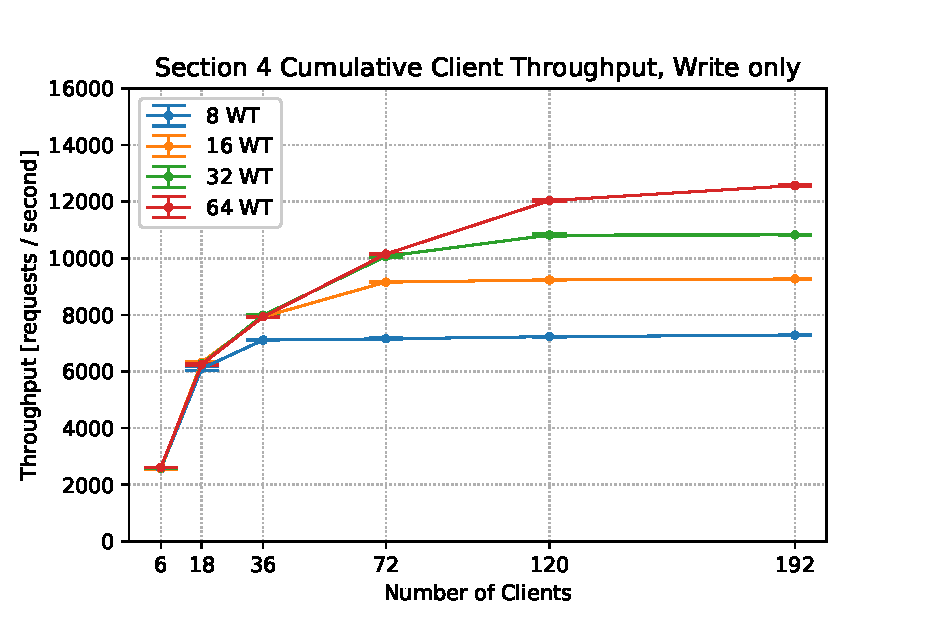
\includegraphics[width=0.7\linewidth]{plots/4b_throughputMiddleware.eps}
    \caption{Throughput of full system, write only, \autoref{sec4}}
    \label{fig:4-throughput}
\end{figure}

\begin{figure}
    \begin{subfigure}{.5\textwidth}
        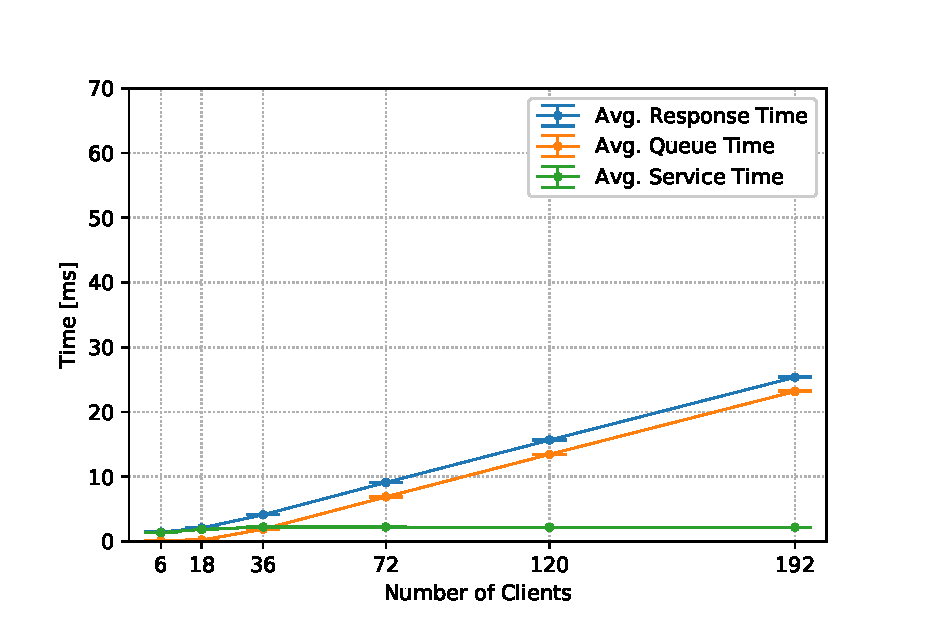
\includegraphics[width=1\linewidth]{plots/4b_extendedLatencyMiddleware_8w.eps}
        \caption{8 worker threads}
    \end{subfigure}
    \begin{subfigure}{.5\textwidth}
        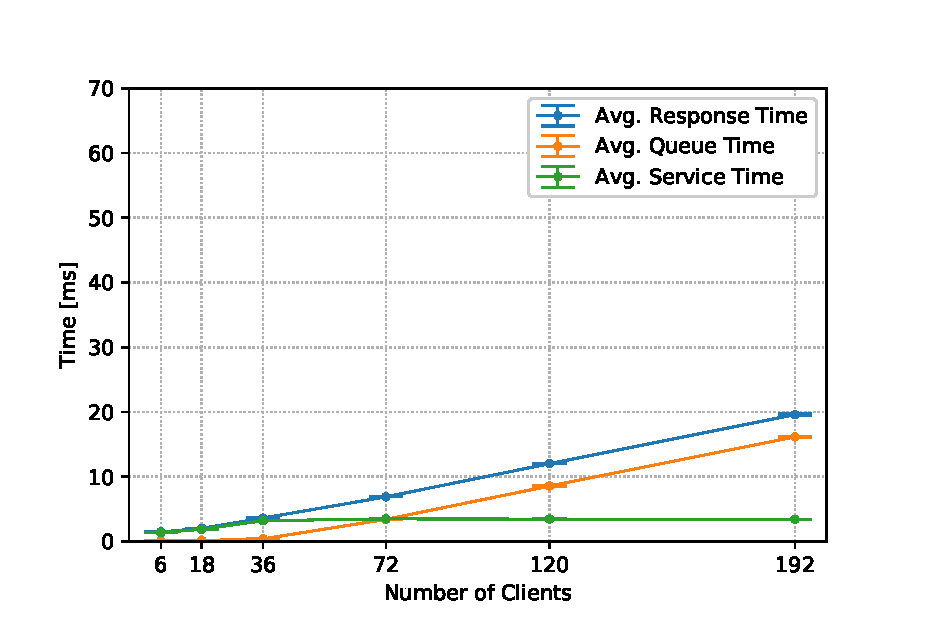
\includegraphics[width=1\linewidth]{plots/4b_extendedLatencyMiddleware_16w.eps}
        \caption{16 worker threads}
    \end{subfigure}
    \begin{subfigure}{.5\textwidth}
        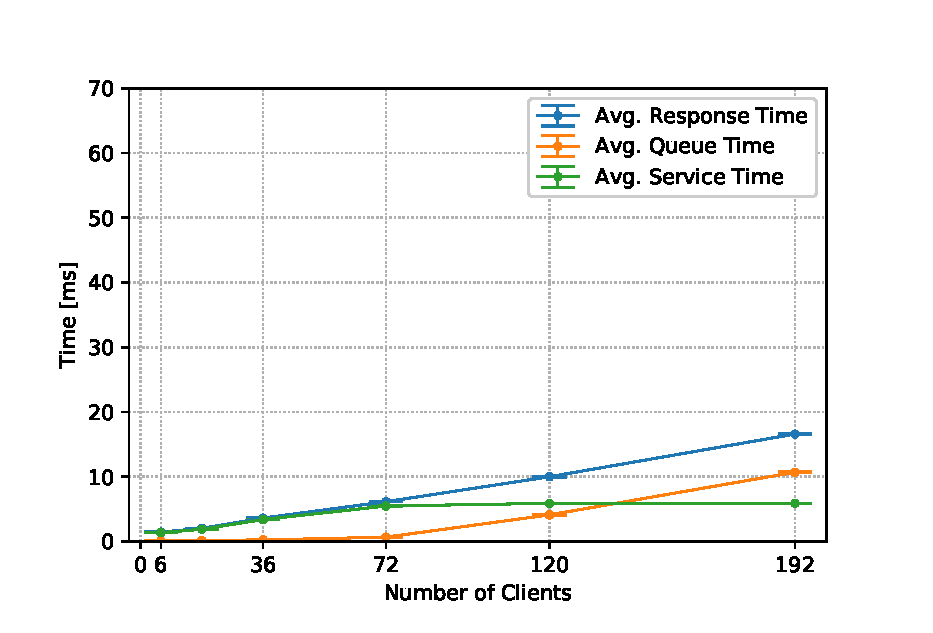
\includegraphics[width=1\linewidth]{plots/4b_extendedLatencyMiddleware_32w.eps}
        \caption{32 worker threads}
    \end{subfigure}
    \begin{subfigure}{.5\textwidth}
        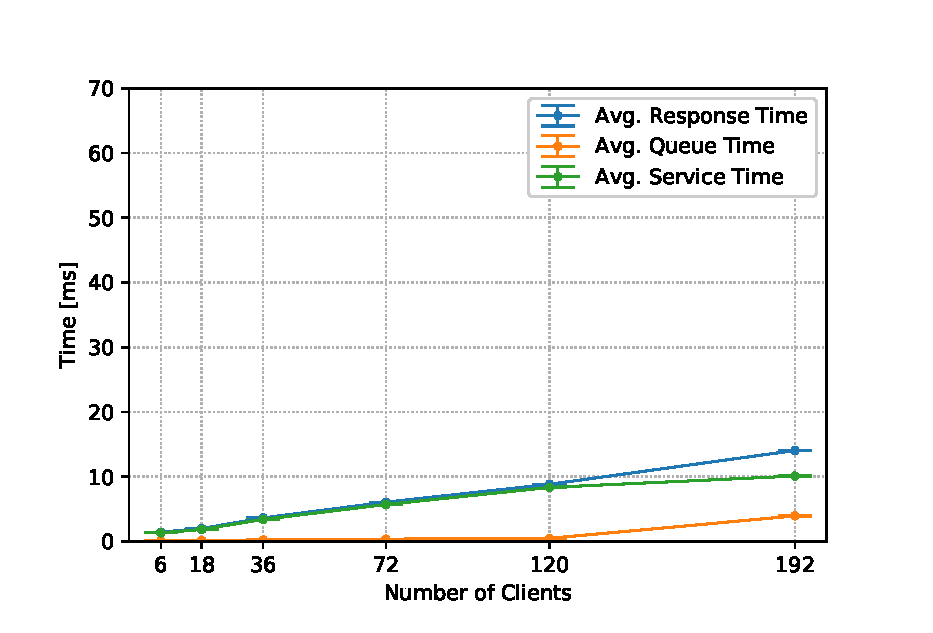
\includegraphics[width=1\linewidth]{plots/4b_extendedLatencyMiddleware_64w.eps}
        \caption{64 worker threads}
    \end{subfigure}

    \caption{Response-, Queue- and Server-Service-Times of full system, Write-only workload for \autoref{sec4}}
    \label{fig:4-times}
\end{figure}
\subsubsection{Explanation}

%Provide a detailed analysis of the results (e.g., bottleneck analysis, component utilizations, average queue lengths, system saturation). Add any additional figures and experiments that help you illustrate your point and support your claims.
Compared to \autoref{sec3.2} there are now 3 servers instead of 1 in the system. For write-only workload the middleware replicates each request to all 3 servers. This comes with some overhead because the middleware needs to send it to each server one by one and receive it one by one. However, this overhead is small compared to the difference in network latency between the servers. The way the middleware is built, it has to wait for the slowest server. \todo{add ping time table to make a point here}
In \autoref{fig:4-throughput} we observe a significantly lower maximum throughput for all worker thread configurations, namely between 12.5 and 20\% less throughput from 8 up to 64 worker threads. When looking at \autoref{fig:4-times} we observe that the total response time slightly higher compared to the one measured in \autoref{sec3.2}. The service time seems to be similar at first, but when inspected in detail we observe that it is slightly higher.
At the maximum throughput configuration for each worker thread configuration (see \autoref{res4}) a difference of the service time (average time waiting for memcached) compared to \autoref{sec3.2} has been measured of 0.33ms, 0.41ms, 0.9ms and 1.5ms for 8, 16, 32 and 64 worker threads respectively. We also observed that the average time in the queue differs also exactly by this time. The amount of requests in the queue has been observed to be similar compared to \autoref{sec3.2}. The higher memcached service time can be explained with the implementation of the middleware and the network structure of the system at hand in mind, where the middleware needs to wait for the response of the slowest memcached server before it can finish a request successfully and start to handle the next one.
\todo{analyze under-saturation and saturation phases}



\subsection{Summary}

\begin{center}
\begin{table}
	\begin{tabular}{|l|p{1.7cm}|p{1.7cm}|p{1.75cm}|p{1.75cm}|}
		\hline                                            & WT=8, 36 clients & WT=16, 72 clients  & WT=32, 120 clients   & WT=64, 192 clients   \\ 
		\hline Throughput (Middleware) [req/s]           & 7110              & 9158                & 10817                 & 12568                 \\ 
		\hline Throughput (Derived from MW response time) [req/s] & 7045       & 9148               & 10810           & 12549         \\
		%8WT, 36cli: 4.11msRT, 1ms thinking time | 16WT, 72cli: 6.87msRT, 1.2ms thinkingtime | 32WT, 120cli: 9.98msRT, 1.1ms thinkingtime \ 64WT, 192cli: 14.04msRT, 1.25ms thinkingtime
		\hline Throughput (Client) [req/s]                & 7108              & 9160                & 10813                 & 12566                 \\ 
		\hline Average time in queue                      & 1.87ms            & 3.39ms              & 4.09ms                & 3.93                  \\ 
		\hline Average length of queue                    & 4.87              & 11.68               & 16.18                 & 19.23                 \\ 
		\hline Average time waiting for memcached         & 2.21ms            & 3.46                & 5.87ms                & 10.09                 \\ 
		\hline 
	\end{tabular}
	\caption{Maximum throughput for the full system in \autoref{sec4}} \label{res4}
\end{table}
\end{center}


\todo{Based on the data provided in these tables, draw conclusions on the state of your system for a variable number of worker threads.}
\section{Gets and Multi-gets (90 pts)}

This section analyzes the effect on throughput and response time of sharding MULTIGET requests.
%For multi-GET workloads, memtier will generate a mixture of SETs, GETs, and multi-GETs. Memtier only allows to specify the maximum number of keys in a multi-GET request. Therefore, be aware that requests can also contain fewer keys than the provided value. It is recommended to record the average size of the multi-GETs. You will have to measure response time on the client as a function of multi-get size, with and without sharding on the middlewares.

\subsection{Sharded Case} \label{sec5.1}

%Run multi-gets with 1, 3, 6 and 9 keys (memtier configuration) with sharding enabled (multi-gets are broken up into smaller multi-gets and spread across servers). Plot average response time as measured on the client, as well as the 25th, 50th, 75th, 90th and 99th 
The results in this section are based on the aggregated request logs from the two middlewares as well as the aggregated output data from the three memtier clients. The first and last three seconds of each of the three repetitions were cut off as startup and cooldown time, leaving 60 seconds of data per repetition. No misses occurred during the test and all client requests were processed and answered. All plots show averages and standard deviations across three repetitions of each configuration. The sanity of the data has been checked with the interactive law for both throughput and response time separately for all configurations and it was found that the interactive law aligns with the measured data. The configurations examined for this section are shown in \autoref{exp5-1} below.


\begin{center}
    \begin{table}
        \centering
    	\begin{tabular}{|l|c|}
    		\hline Number of servers                & 3                       \\ 
    		\hline Number of client machines        & 3                       \\ 
    		\hline Instances of memtier per machine & 2                       \\ 
    		\hline Threads per memtier instance     & 1                       \\
    		\hline Virtual clients per thread       & 2     		            \\ 
    		\hline Workload                         & ratio=1:$<$Multi-Get size$>$             \\
    		\hline Multi-Get behavior               & Sharded                 \\
    		\hline Multi-Get size                   & [1, 3, 6, 9]            \\
    		\hline Number of middlewares            & 2                       \\
    		\hline Worker threads per middleware    & 64                      \\
    		\hline Repetitions                      & 3                       \\ 
    		\hline 
    	\end{tabular}
    	\caption{Experiment configurations for \autoref{sec5.1}} \label{exp5-1}
    \end{table}
\end{center}

\begin{figure}
    \begin{subfigure}{.5\textwidth}
        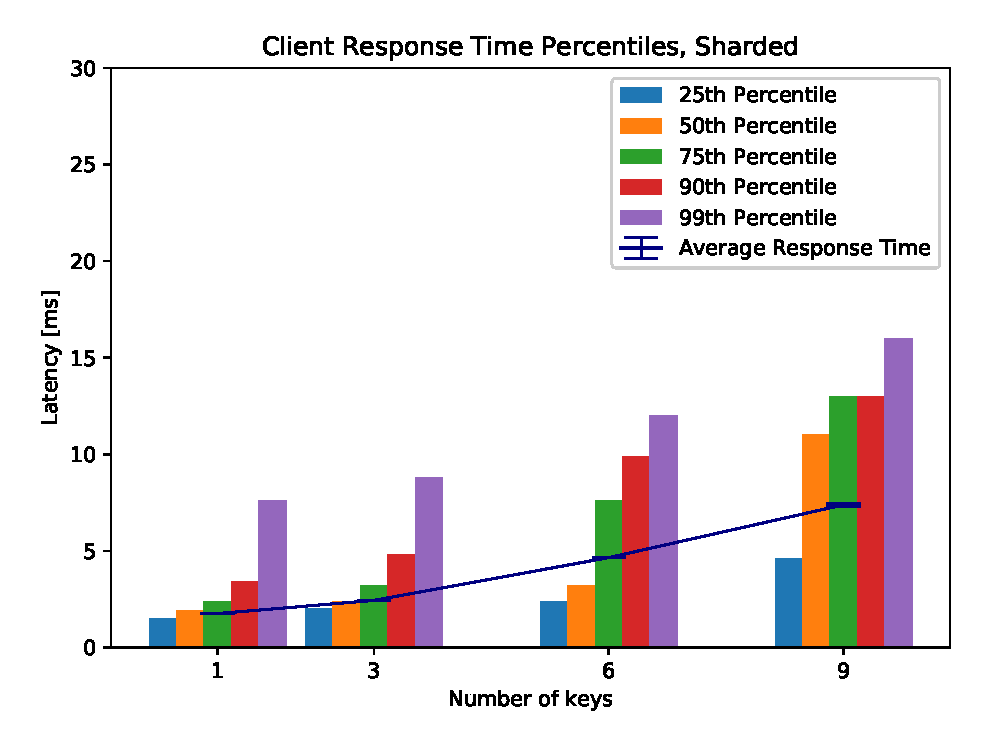
\includegraphics[width=1\linewidth]{plots/logSection5c_latencyPercentilesMemtier.eps}
        \caption{Sharded}
    \end{subfigure}
    \begin{subfigure}{.5\textwidth}
        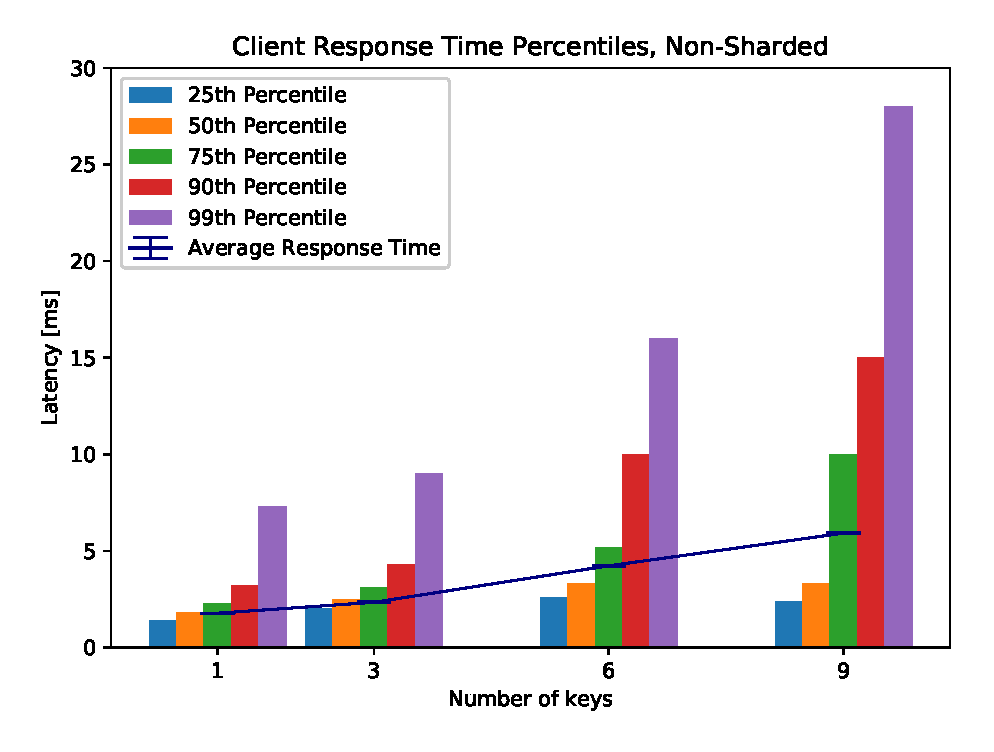
\includegraphics[width=1\linewidth]{plots/logSection5d_latencyPercentilesMemtier.eps}
        \caption{Non-Sharded}
    \end{subfigure}

    \caption{Response time and percentiles measured on the client side, sections 5.1 and 5.2}
    \label{fig:5-latencyPercentiles}
\end{figure}


\subsubsection{Explanation}
%Provide a detailed analysis of the results (e.g., bottleneck analysis, component utilizations, average queue lengths, system saturation). Add any additional figures and experiments that help you illustrate your point and support your claims.

\subsection{Non-sharded Case} \label{sec5.2}
%Run multi-gets with 1, 3, 6 and 9 keys (memtier configuration) with sharding disabled. Plot average response time as measured on the client, as well as the 25th, 50th, 75th, 90th and 99th percentiles.
The results in this section are based on the aggregated request logs from the two middlewares as well as the aggregated output data from the three memtier clients. The first and last three seconds of each of the three repetitions were cut off as startup and cooldown time, leaving 60 seconds of data per repetition. No misses occurred during the test and all client requests were processed and answered. All plots show averages and standard deviations across three repetitions of each configuration. The sanity of the data has been checked with the interactive law for both throughput and response time separately for all configurations and it was found that the interactive law aligns with the measured data. The configurations examined for this section are shown in \autoref{exp5-2} below.

\begin{center}
    \begin{table}
        \centering
    	\begin{tabular}{|l|c|}
    		\hline Number of servers                & 3                            \\ 
    		\hline Number of client machines        & 3                            \\ 
    		\hline Instances of memtier per machine & 2                            \\ 
    		\hline Threads per memtier instance     & 1                            \\
    		\hline Virtual clients per thread       & 2                		       \\ 
    		\hline Workload                         & ratio=1:$<$Multi-Get size$>$ \\
    		\hline Multi-Get behavior               & Non-Sharded                  \\
    		\hline Multi-Get size                   & [1, 3, 6 9]                  \\
    		\hline Number of middlewares            & 2                            \\
    		\hline Worker threads per middleware    & 64                           \\
    		\hline Repetitions                      & 3                            \\ 
    		\hline 
    	\end{tabular}
    	\caption{Experiment configurations for \autoref{sec5.2}} \label{exp5-2}
    \end{table}
\end{center}

\begin{figure}
    \centering
    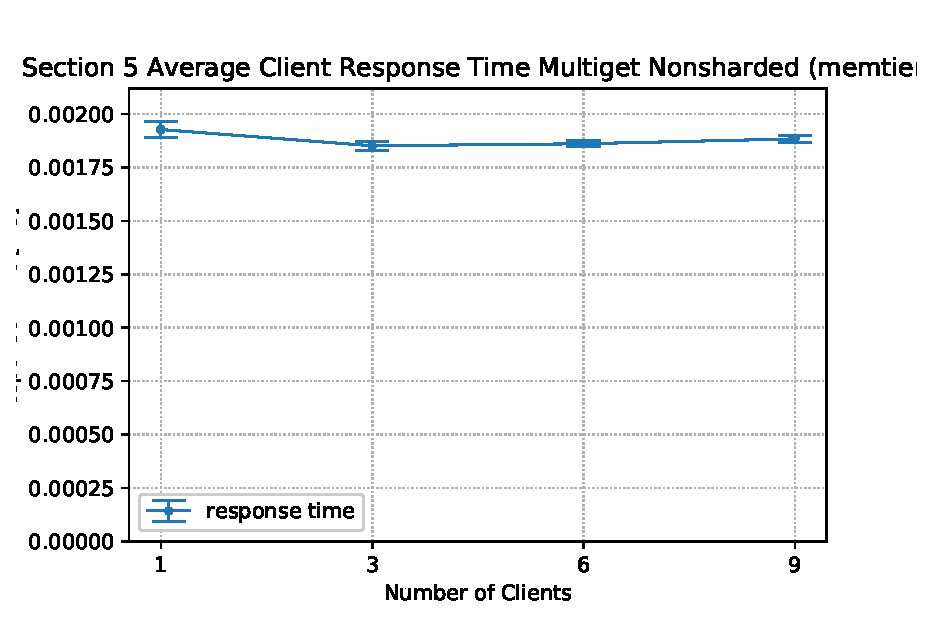
\includegraphics[width=0.7\linewidth]{plots/5b_latencyMemtier.eps}
    \caption{Response time measured on the client, non-sharded}
    \label{fig:5-2-responsetime}
\end{figure}

\subsubsection{Explanation}

%Provide a detailed analysis of the results (e.g., bottleneck analysis, component utilizations, average queue lengths, system saturation). Add any additional figures and experiments that help you illustrate your point and support your claims.
\todo{elaborate on non-sharded histograms and percentiles}

\subsection{Histogram}
%For the case with 6 keys inside the multi-get, display four histograms representing the sharded and non-sharded response time distribution, both as measured on the client, and inside the middleware. Choose the bucket size in the same way for all four, and such that there are at least 10 buckets on each of the graphs.
\autoref{fig:5-1:Histograms} shows histograms for both memtier and middleware both for a sharded and a non-sharded configuration. The histograms were generated using the data from \autoref{sec5.1} and \autoref{sec5.2} for the configuration of memtier where 6 key MULTIGET requests were sent. For sharded and non-sharded independently we observe a shift from memtier to middleware, namely the histogram of the middleware is shifted 1 bucket to the right, meaning the response times measured at the client are around 1ms longer. This can be explained with the additional round-trip time of each request from client to middleware. The middleware measures its response time from the arrival of the request until before it is returned to the client, so we expect the response time to be 1 round-trip time off compared to the response time measured at the client. Looking at the histogram and the mean ping time of 1ms this hypothesis is confirmed.
\todo{further explain differences between sharded vs non-sharded }



\begin{figure}
    \begin{subfigure}{.5\textwidth}
        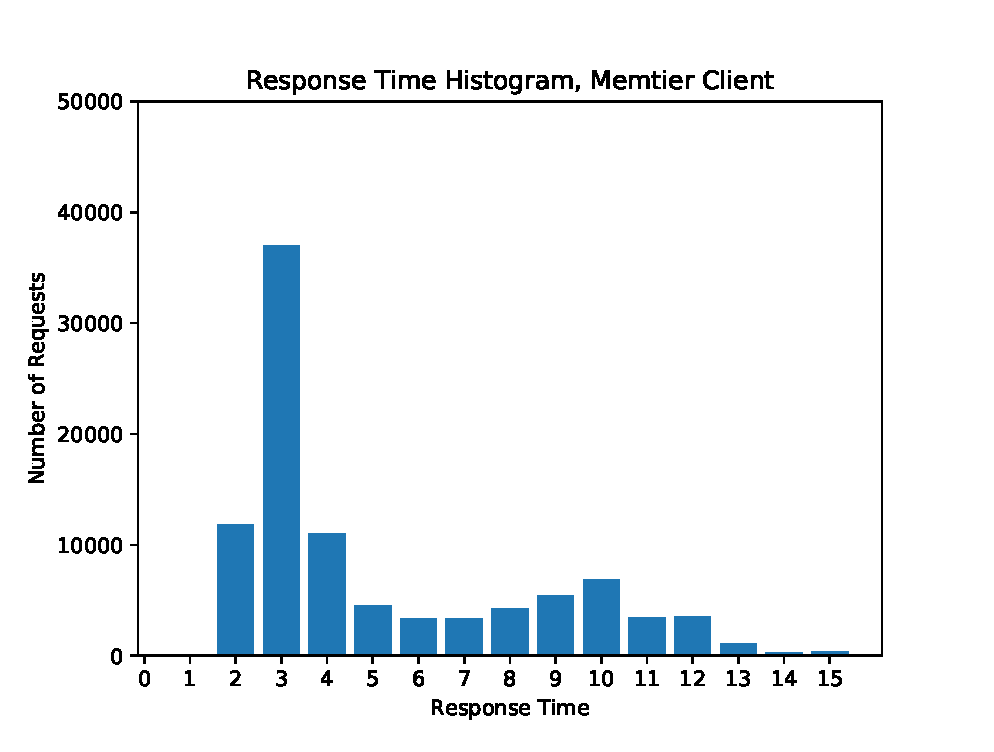
\includegraphics[width=1\linewidth]{plots/logSection5c_histogramMemtier.eps}
        \caption{Memtier, Sharded}
    \end{subfigure}
    \begin{subfigure}{.5\textwidth}
        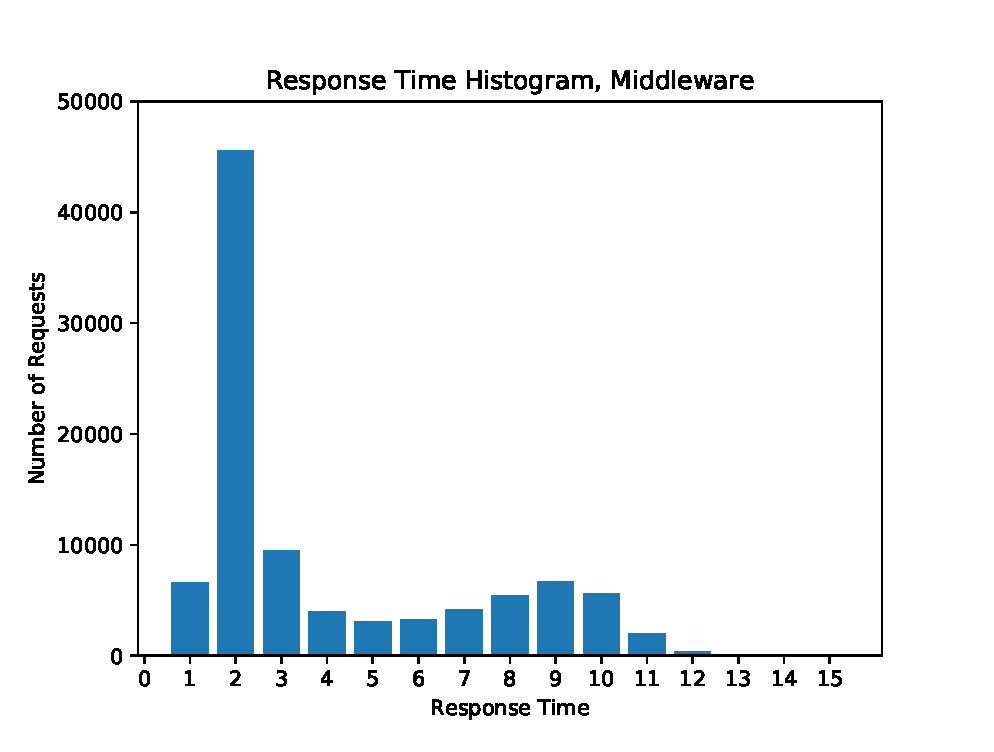
\includegraphics[width=1\linewidth]{plots/logSection5c_histogramMiddleware.eps}
        \caption{Middleware, Sharded}
    \end{subfigure}

    \begin{subfigure}{.5\textwidth}
        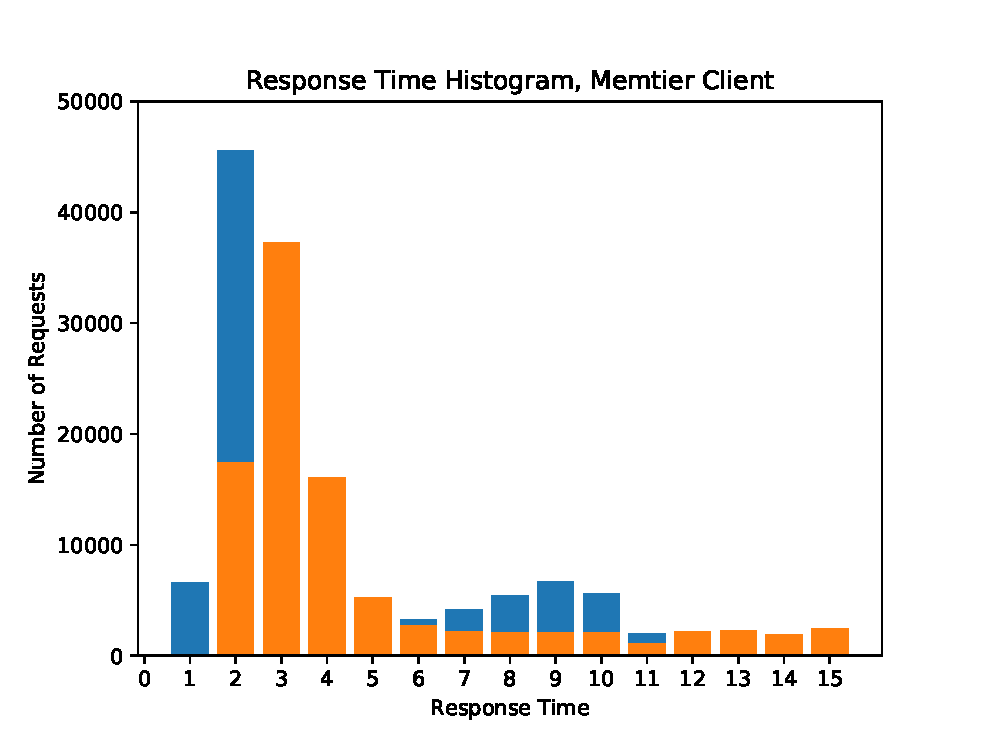
\includegraphics[width=1\linewidth]{plots/logSection5d_histogramMemtier.eps}
        \caption{Memtier, Non-Sharded}
    \end{subfigure}
    \begin{subfigure}{.5\textwidth}
        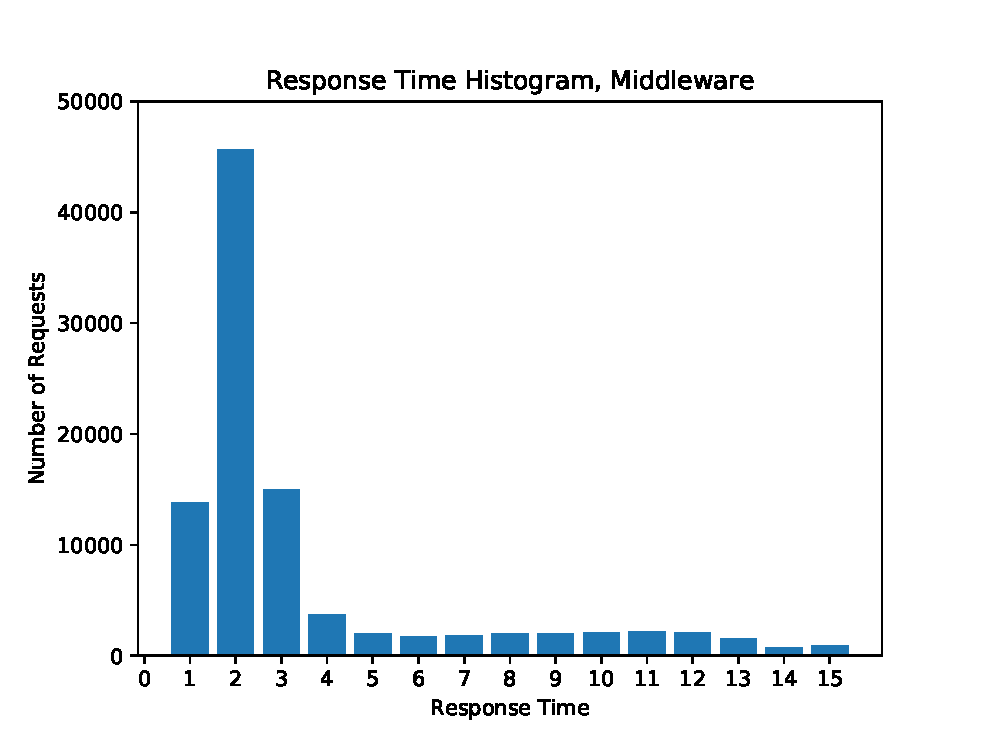
\includegraphics[width=1\linewidth]{plots/logSection5d_histogramMiddleware.eps}
        \caption{Middleware, Non-Sharded}
    \end{subfigure}
    \caption{Response Time Histograms}
    \label{fig:5-1:Histograms}
\end{figure}

\subsection{Summary}

Provide a detailed comparison of the sharded and non-shareded modes. For which multi-GET size is sharding the preferred option? Provide a detailed analysis of your system. Add any additional figures and experiments that help you illustrate your point and support your claims.

\section{2K Analysis (90 pts)}

In this section, a 2k analysis for k=3 is being performed. With this, the impact of the number of memcached servers, the number of worker threads and the number of middlewares (as well as any combination of these) on throughput and response time is derived. The following parameter choices are being investigated:

\begin{itemize}
		
	\item Worker threads per MW $x_a \in \{8, 32\}$
	\item Number of memcached servers $x_b \in \{1, 3\}$
	\item Number of middlewares $x_c \in \{1,2\}$
	      	      
\end{itemize}

Repeat the experiment for (a)~a write-only and (b)~a read-only workload.
For each of the two workloads, what is the impact of these parameters on throughput, respectively response time?

\begin{center}
	\scriptsize{
		\begin{tabular}{|l|c|}
			\hline Number of servers                & 1 and 3                                     \\ 
			\hline Number of client machines        & 3                                           \\ 
			\hline Instances of memtier per machine & 1 (1 middleware) or 2 (2 middlewares)       \\ 
			\hline Threads per memtier instance     & 2 (1 middleware) or 1 (2 middlewares)       \\
			\hline Virtual clients per thread       & 32                                          \\ 
			\hline Workload                         & Write-only and Read-only                    \\
			\hline Number of middlewares            & 1 and 2                                     \\
			\hline Worker threads per middleware    & 8 and 32                                    \\
			\hline Repetitions                      & 3                                   \\ 
			\hline 
		\end{tabular}
	} 
\end{center}

\subsection{Read-only Workload}

\autoref{2k:read-only} shows parameters and combinations of them, measured throughput and response time, allocation of variance and derived effect sizes under a read-only workload. The additive 2k factorial design has been used because no multiplicative effects have been observed.
- clearly, server is bottleneck. dstat confirms this assumption as well, 12.5MB/S avg upload per server
- throughput and response time must be in close relationship. It is expected that factors that strongly influence throughput inversely influence response time in an equally strong way.
- refer to section 2 / 3
\todo{compactify, just mention the effect and allocation of Variance. See example from Valentin}

\begin{table}
    \begin{subtable}{1.0\linewidth}\centering
        {\begin{tabular}{|cccccccc|cc|}
            \hline
            $I$ & $x_a$ & $x_b$ & $x_c$ & $x_{ab}$ & $x_{bc}$ & $x_{ac}$ & $x_{abc}$ & $y_{mean}$ & $y_{stddev}$\\
            \hline
                    1 &     -1 &       -1 &     -1 &      1 &      1 &       1 &      -1 & 2936.411 &   0.904 \\
                    1 &     -1 &       -1 &      1 &      1 &     -1 &      -1 &       1 & 2941.454 &   3.843 \\
                    1 &     -1 &        1 &     -1 &     -1 &     -1 &       1 &       1 & 8702.579 &  26.966 \\
                    1 &     -1 &        1 &      1 &     -1 &      1 &      -1 &      -1 & 8803.022 &   3.089 \\
                    1 &      1 &       -1 &     -1 &     -1 &      1 &      -1 &       1 & 2940.514 &   2.471 \\
                    1 &      1 &       -1 &      1 &     -1 &     -1 &       1 &      -1 & 2942.596 &   0.192 \\
                    1 &      1 &        1 &     -1 &      1 &     -1 &      -1 &      -1 & 8804.268 &   2.778 \\
                    1 &      1 &        1 &      1 &      1 &      1 &       1 &       1 & 8797.934 &  24.191 \\
            \hline
            $q_0$ & $q_a$ & $q_b$ & $q_c$ & $q_{ab}$ & $q_{bc}$ & $q_{ac}$ & $q_{abc}$ & - & -\\
              5858.597 & 12.731 & 2918.354 & 12.654 & 11.419 & 10.873 & -13.717 & -12.977 & /8 & - \\
            \hline
        \end{tabular}
        \caption{Parameters and Effect Sizes, Throughput}}
    \end{subtable}
    \begin{subtable}{1.0\linewidth}\centering
        {\begin{tabular}{|cccccccc|}
            \hline
            $q_a$ & $q_b$ & $q_c$ & $q_{ab}$ & $q_{bc}$ & $q_{ac}$ & $q_{abc}$ & Error \\
            \hline
            0.002\% & 99.989\% & 0.002\% & 0.002\%   &  0.001\%   &   0.002\%  &   0.002\%   & 0.000\% \\
            \hline
        \end{tabular}
        \caption{Allocation of Variance, Throughput}}
    \end{subtable}

    \begin{subtable}{1.0\linewidth}\centering
        {\begin{tabular}{|cccccccc|cc|}
            \hline
            $I$ & $x_a$ & $x_b$ & $x_c$ & $x_{ab}$ & $x_{bc}$ & $x_{ac}$ & $x_{abc}$ & $y_{mean}$ & $y_{stddev}$\\
            \hline
                  1 &     -1 &      -1 &     -1 &      1 &      1 &     1 &    -1 & 64.356 &   0.033 \\
                  1 &     -1 &      -1 &      1 &      1 &     -1 &    -1 &     1 & 64.188 &   0.094 \\
                  1 &     -1 &       1 &     -1 &     -1 &     -1 &     1 &     1 & 21.098 &   0.073 \\
                  1 &     -1 &       1 &      1 &     -1 &      1 &    -1 &    -1 & 20.802 &   0.013 \\
                  1 &      1 &      -1 &     -1 &     -1 &      1 &    -1 &     1 & 63.904 &   0.047 \\
                  1 &      1 &      -1 &      1 &     -1 &     -1 &     1 &    -1 & 63.966 &   0.002 \\
                  1 &      1 &       1 &     -1 &      1 &     -1 &    -1 &    -1 & 20.528 &   0.004 \\
                  1 &      1 &       1 &      1 &      1 &      1 &     1 &     1 & 20.611 &   0.077 \\
            \hline
            $q_0$ & $q_a$ & $q_b$ & $q_c$ & $q_{ab}$ & $q_{bc}$ & $q_{ac}$ & $q_{abc}$ & - & -\\
             42.431 & -0.179 & -21.672 & -0.040 & -0.011 & -0.013 & 0.076 & 0.019 &      /8 &       - \\
            \hline
        \end{tabular}
        \caption{Parameters and Effect Sizes, Response Time}}
    \end{subtable}
    \begin{subtable}{1.0\linewidth}\centering
       {\begin{tabular}{|cccccccc|}
            \hline
            $q_a$ & $q_b$ & $q_c$ & $q_{ab}$ & $q_{bc}$ & $q_{ac}$ & $q_{abc}$ & Error \\
            \hline
              0.007\% &  99.991\% &  0.000\% &  0.000\% &  0.000\% & 0.001\% & 0.000\% &  0.001\% \\
            \hline
        \end{tabular}
        \caption{Allocation of Variance, Response Time}}
    \end{subtable}

    \caption{2K Analysis, Read-only Workload}
    \label{2k:read-only}
\end{table}

\subsection{Write-only Workload}
\autoref{2k:write-only} shows parameters and combinations of them, measured throughput and response time, allocation of variance and derived effect sizes under a write-only workload. The additive 2k factorial design has been used because no multiplicative effects have been observed. We observe that for write-only workload $x_a$, the number of worker threads has the most significant effect on the system followed by the number of middlewares $x_c$. This aligns with the observations in sections 3 and 4 for write-only workload where we observed that the middleware is the bottleneck due to too few worker threads. The reason for $x_a$ having a significantly higher allocation of variance in comparison to $x_c$ is, that the number of worker threads is increased by a factor of 4 with $x_a$ while it is only doubled with $x_c$.
The number of memcached servers, $x_b$, has the lowest effect for write-only workload and the effect on the throughput is negative, meaning increasing the amount of servers from 1 to 3 actually leads to a decrease of throughput and an increase of latency. 
As we have seen in previous chapters \todo{be more specific here}, the decrease of throughput for write-only workload can be explained with reference to the implementation of the middleware. The middleware sends SET requests to each memcached server and responses are received from each server one by one. Besides the sending and receiving, the main difference in response time comes from the dependence on the slowest server response time. \todo{name concrete values here}.
%This makes sense because for write-only workload the servers do not need to send massive amounts of data but only receive and store. The bottleneck this time lies in the middleware, where we can even observe the maximum outgoing link capacity of 100MB/s being reached for the configuration with 1 middleware and 3 servers.
\todo{mention other chapters, link to chaper 2/3/4}

\begin{table}
    \begin{subtable}{1.0\linewidth}\centering
        {\begin{tabular}{|cccccccc|cc|}
            \hline
            $I$ & $x_a$ & $x_b$ & $x_c$ & $x_{ab}$ & $x_{bc}$ & $x_{ac}$ & $x_{abc}$ & $y_{mean}$ & $y_{stddev}$\\
            \hline
                    1 &       -1 &       -1 &       -1 &        1 &      1 &       1 &    -1 &  6820.136 &  16.917 \\
                    1 &       -1 &       -1 &        1 &        1 &     -1 &      -1 &     1 &  8557.913 &  38.062 \\
                    1 &       -1 &        1 &       -1 &       -1 &     -1 &       1 &     1 &  5333.355 & 174.900 \\
                    1 &       -1 &        1 &        1 &       -1 &      1 &      -1 &    -1 &  7240.880 &  35.038 \\
                    1 &        1 &       -1 &       -1 &       -1 &      1 &      -1 &     1 & 10573.918 &  23.666 \\
                    1 &        1 &       -1 &        1 &       -1 &     -1 &       1 &    -1 & 13065.804 &  12.610 \\
                    1 &        1 &        1 &       -1 &        1 &     -1 &      -1 &    -1 &  8110.258 &  15.192 \\
                    1 &        1 &        1 &        1 &        1 &      1 &       1 &     1 & 10789.416 &  59.709 \\
            \hline
            $q_0$ & $q_a$ & $q_b$ & $q_c$ & $q_{ab}$ & $q_{bc}$ & $q_{ac}$ & $q_{abc}$ & - & -\\
             8811.460 & 1823.389 & -942.983 & 1102.043 & -242.029 & 44.627 & 190.718 & 2.190 &  /8 &       - \\
            \hline
        \end{tabular}
        \caption{Parameters and Effect Sizes, Throughput}}
    \end{subtable}
    \begin{subtable}{1.0\linewidth}\centering
        {\begin{tabular}{|cccccccc|}
            \hline
            $q_a$ & $q_b$ & $q_c$ & $q_{ab}$ & $q_{bc}$ & $q_{ac}$ & $q_{abc}$ & Error \\
            \hline
            60.172\% &   16.093\% &   21.980\% &    1.060\% &  0.036\% &   0.658\% & 0.000\% &     0.000\% \\
            \hline
        \end{tabular}
        \caption{Allocation of Variance, Throughput}}
    \end{subtable}

    \begin{subtable}{1.0\linewidth}\centering
        {\begin{tabular}{|cccccccc|cc|}
            \hline
            $I$ & $x_a$ & $x_b$ & $x_c$ & $x_{ab}$ & $x_{bc}$ & $x_{ac}$ & $x_{abc}$ & $y_{mean}$ & $y_{stddev}$\\
            \hline
                  1 &     -1 &     -1 &     -1 &      1 &      1 &     1 &    -1 & 27.219 &   0.061 \\
                  1 &     -1 &     -1 &      1 &      1 &     -1 &    -1 &     1 & 21.378 &   0.045 \\
                  1 &     -1 &      1 &     -1 &     -1 &     -1 &     1 &     1 & 35.060 &   1.193 \\
                  1 &     -1 &      1 &      1 &     -1 &      1 &    -1 &    -1 & 25.521 &   0.140 \\
                  1 &      1 &     -1 &     -1 &     -1 &      1 &    -1 &     1 & 16.914 &   0.032 \\
                  1 &      1 &     -1 &      1 &     -1 &     -1 &     1 &    -1 & 13.575 &   0.050 \\
                  1 &      1 &      1 &     -1 &      1 &     -1 &    -1 &    -1 & 21.570 &   0.091 \\
                  1 &      1 &      1 &      1 &      1 &      1 &     1 &     1 & 16.604 &   0.092 \\
            \hline
            $q_0$ & $q_a$ & $q_b$ & $q_c$ & $q_{ab}$ & $q_{bc}$ & $q_{ac}$ & $q_{abc}$ & - & -\\
             22.230 & -5.064 &  2.459 & -2.961 & -0.537 & -0.666 & 0.885 & 0.259 &  /8 &       - \\
            \hline
        \end{tabular}
        \caption{Parameters and Effect Sizes, Response Time}}
    \end{subtable}
    \begin{subtable}{1.0\linewidth}\centering
       {\begin{tabular}{|cccccccc|}
            \hline
            $q_a$ & $q_b$ & $q_c$ & $q_{ab}$ & $q_{bc}$ & $q_{ac}$ & $q_{abc}$ & Error \\
            \hline
            60.745\% & 14.316\% & 20.760\% &  0.684\% &  1.049\% & 1.853\% & 0.159\% &  0.435\% \\
            \hline
        \end{tabular}
        \caption{Allocation of Variance, Response Time}}
    \end{subtable}

    \caption{2K Analysis, Write-only Workload}
    \label{2k:write-only}
\end{table}


\section{Queuing Model (90 pts)}

Note that for queuing models it is enough to use the experimental results from the previous sections. It is, however, possible that the numbers you need are not only the ones in the figures we asked for, but also the internal measurements that you have obtained through instrumentation of your middleware.

\subsection{M/M/1} \label{sec7.1}

%Build queuing model based on Section 4 (write-only throughput) for each worker-thread configuration of the middleware. Use one M/M/1 queue to model your entire system. Motivate your choice of input parameters to the model. Explain for which experiments the predictions of the model match and for which they do not.
\begin{figure}
    \begin{subfigure}{.5\textwidth}
        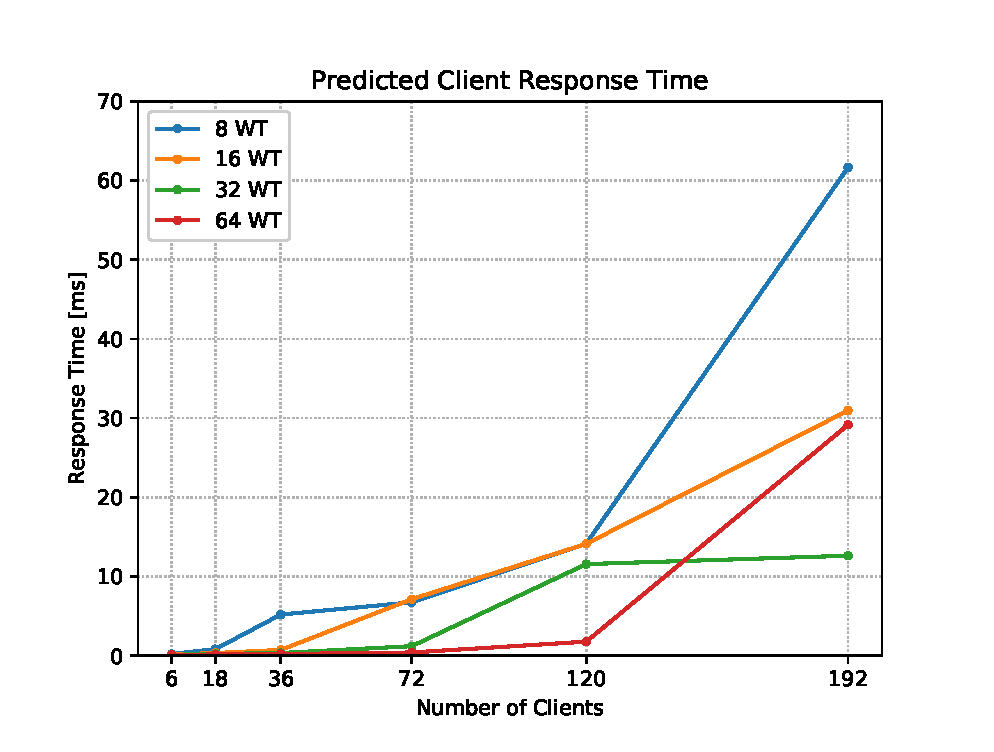
\includegraphics[width=1\linewidth]{plots/7_MM1_ResponseTimePredicted.eps}
    \end{subfigure}
    \begin{subfigure}{.5\textwidth}
        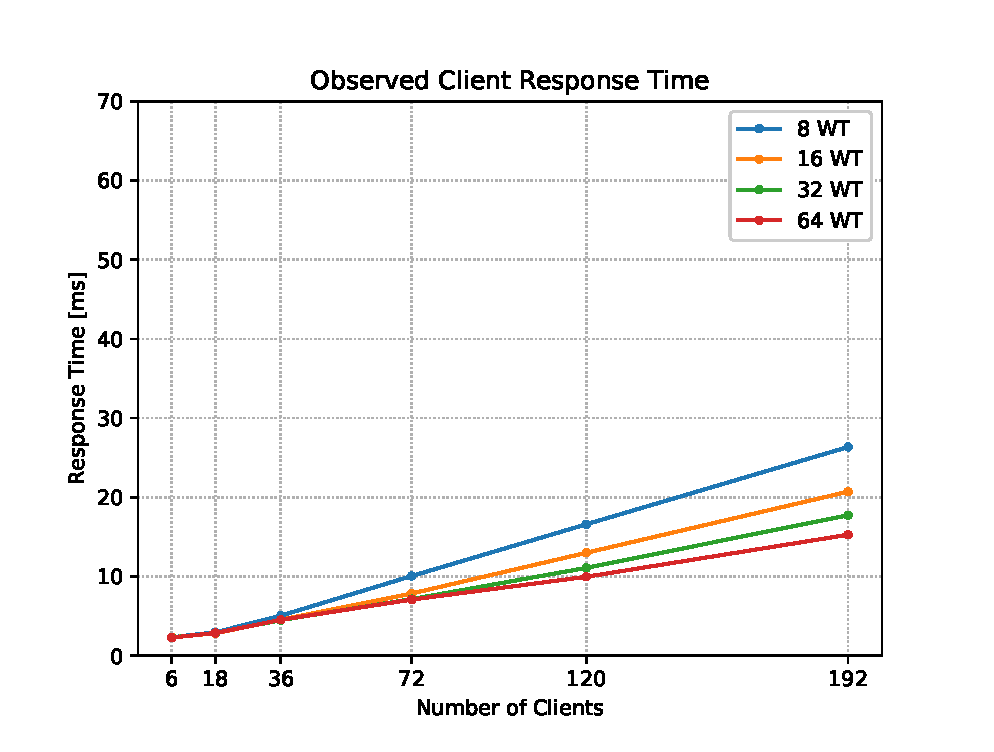
\includegraphics[width=1\linewidth]{plots/7_MM1_ResponseTimeObserved.eps}
    \end{subfigure}
    \caption{M/M/1 predicted and measured Response Times, Full System, \autoref{sec7.1}}
    \label{fig:mm1-RT}
\end{figure}

\begin{figure}
    \begin{subfigure}{.5\textwidth}
        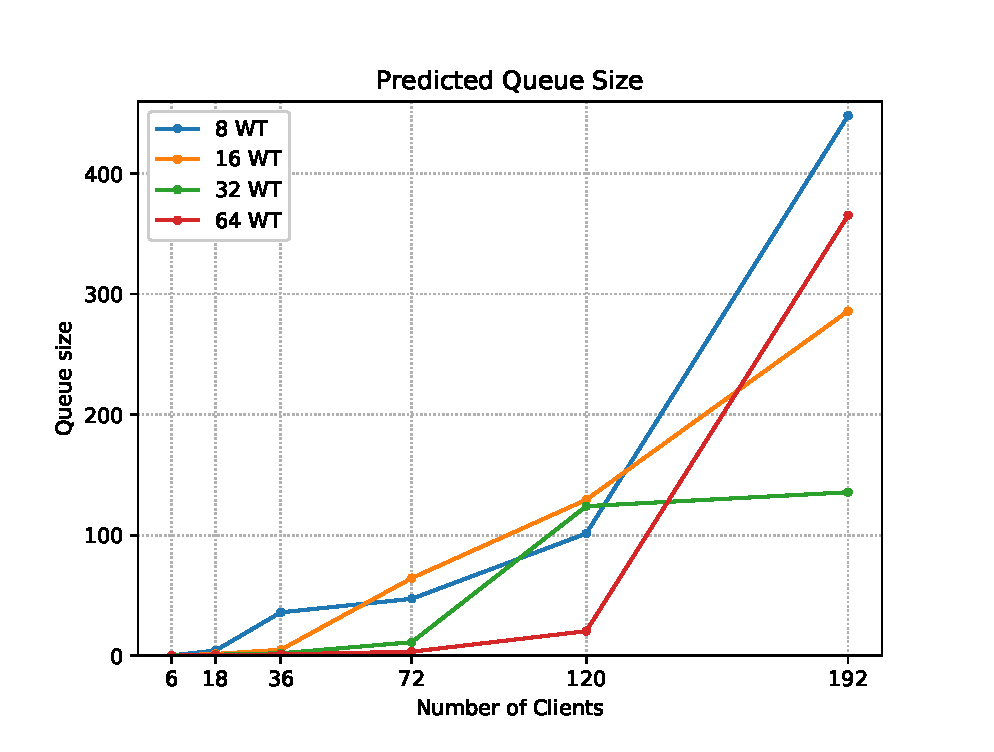
\includegraphics[width=1\linewidth]{plots/7_MM1_QueueSizePred.eps}
    \end{subfigure}
    \begin{subfigure}{.5\textwidth}
        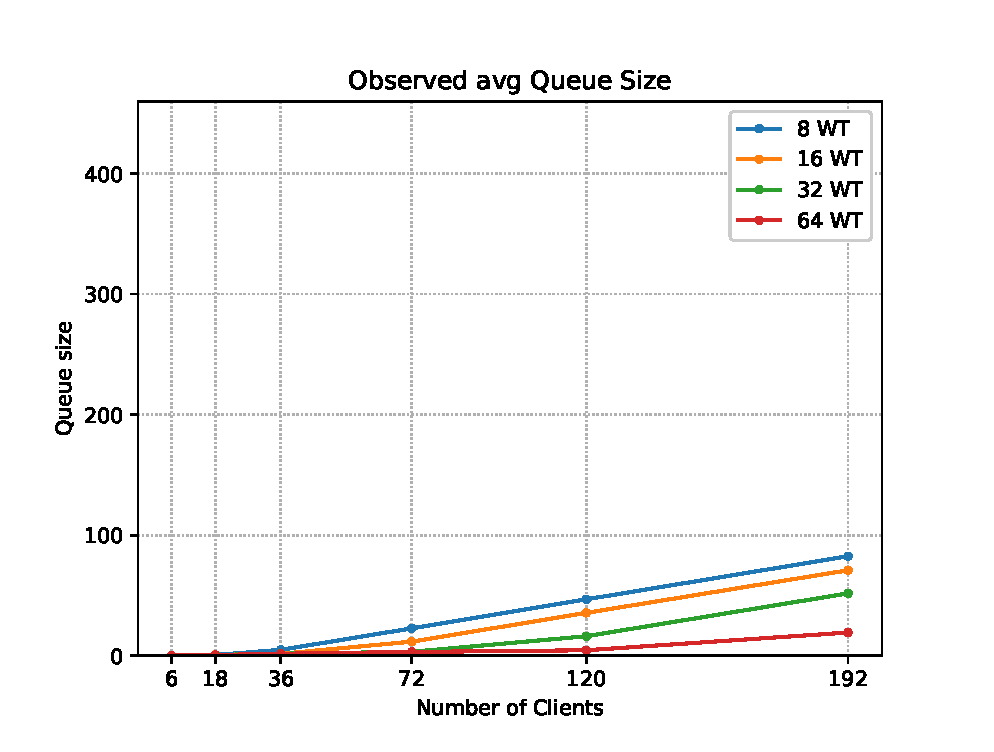
\includegraphics[width=1\linewidth]{plots/7_MM1_QueueSizeObserved.eps}
    \end{subfigure}
    \caption{M/M/1 predicted and measured Queue Size, Full System, \autoref{sec7.1}}
    \label{fig:mm1-queueLen}
\end{figure}
- model too simplistic. In our model it is not possible that more than numClients requests are in queue, in model this is possible


\begin{table}
    \begin{subtable}{1.0\linewidth}\centering
        \begin{tabular}{lrrlll}
        \hline
        \# Clients &  $\lambda$&  $\rho$& $E[r]$&        $E[n\_q]$& $E[w]$\\
        \hline
          6 &    2571.91 &    0.35 &    0.21 // 2.33 &     0.19 // 0.11 &    0.07 // 0.07 \\
         18 &    6093.61 &    0.83 &    0.83 // 2.95 &     4.22 // 0.62 &    0.69 // 0.20 \\
         36 &    7107.66 &    0.97 &    5.20 // 5.06 &    35.98 // 4.87 &    5.06 // 1.87 \\
         72 &    7151.63 &    0.98 &   6.74 // 10.06 &   47.22 // 22.71 &    6.60 // 6.86 \\
        120 &    7229.38 &    0.99 &  14.16 // 16.59 &  101.38 // 46.78 &  14.02 // 13.44 \\
        192 &    7283.78 &    1.00 &  61.66 // 26.35 &  448.10 // 82.55 &  61.52 // 23.17 \\
        \hline
        \end{tabular}
        \caption{8 Worker Threads, $\mu = 7300 ops/s$}
    \end{subtable}
    \begin{subtable}{1.0\linewidth}\centering
        \begin{tabular}{lrrlll}
        \hline
        \# Clients &  $\lambda$&  $\rho$& $E[r]$&        $E[n\_q]$& $E[w]$\\
        \hline
          6 &    2577.76 &    0.28 &    0.15 // 2.32 &     0.11 // 0.11 &    0.04 // 0.07 \\
         18 &    6330.40 &    0.68 &    0.34 // 2.84 &     1.45 // 0.70 &    0.23 // 0.12 \\
         36 &    7930.72 &    0.85 &    0.73 // 4.53 &     4.94 // 1.58 &    0.62 // 0.38 \\
         72 &    9159.92 &    0.98 &    7.14 // 7.85 &   64.40 // 11.68 &    7.03 // 3.39 \\
        120 &    9229.22 &    0.99 &  14.13 // 13.00 &  129.41 // 35.57 &   14.02 // 8.55 \\
        192 &    9267.70 &    1.00 &  30.96 // 20.71 &  285.92 // 70.90 &  30.85 // 16.13 \\
        \hline
        \end{tabular}
        \caption{16 Worker Threads, $\mu = 9300 ops/s$}
    \end{subtable}
    
    \begin{subtable}{1.0\linewidth}\centering
        \begin{tabular}{lrrlll}
        \hline
        \# Clients &  $\lambda$&  $\rho$& $E[r]$&        $E[n\_q]$& $E[w]$\\
        \hline
          6 &    2596.04 &    0.24 &    0.12 // 2.31 &     0.07 // 0.10 &    0.03 // 0.07 \\
         18 &    6274.84 &    0.58 &    0.22 // 2.86 &     0.78 // 0.66 &    0.12 // 0.12 \\
         36 &    7991.58 &    0.73 &    0.34 // 4.50  &     2.01 // 1.67 &    0.25 // 0.21 \\
         72 &   10070.24 &    0.92 &    1.21 // 7.14 &    11.21 // 3.22 &    1.11 // 0.65 \\
        120 &   10813.54 &    0.99 &  11.57 // 11.09 &  124.08 // 16.18 &   11.47 // 4.09 \\
        192 &   10820.80 &    0.99 &  12.63 // 17.74 &  135.63 // 51.73 &  12.53 // 10.68 \\
        \hline
        \end{tabular}
        \caption{32 Worker Threads, $\mu = 10900 ops/s$}
    \end{subtable}
    
    \begin{subtable}{1.0\linewidth}\centering
        \begin{tabular}{lrrlll}
        \hline
        \# Clients &  $\lambda$&  $\rho$& $E[r]$&        $E[n\_q]$&        $E[w]$\\
        \hline
          6 &    2611.63 &    0.21 &    0.10 // 2.29 &     0.05 // 0.10 &   0.02 // 0.07 \\
         18 &    6262.69 &    0.50 &    0.16 // 2.87 &     0.49 // 0.60 &   0.08 // 0.12 \\
         36 &    7933.14 &    0.63 &    0.21 // 4.53 &     1.07 // 1.62 &   0.13 // 0.21 \\
         72 &   10147.69 &    0.81 &    0.41 // 7.09 &     3.33 // 3.13 &   0.33 // 0.34 \\
        120 &   12036.31 &    0.96 &    1.77 // 9.96 &    20.40 // 4.52 &   1.69 // 0.46 \\
        192 &   12565.70 &    1.00 &  29.16 // 15.27 &  365.40 // 19.24 &  29.08 // 3.93 \\
        \hline
        \end{tabular}
        \caption{64 Worker Threads, $\mu = 12600 ops/s$}
    \end{subtable}

    \caption{System Properties, M/M/1 Model. Please note that in the three rightmost columns the values are displayed as $predicted  //  observed$. $E[r]$ is the response time in ms,  $E[n\_q]$ displays the number of requests in the queue and $E[w]$ displays is the queue waiting time in ms. }
    \label{mm1}
\end{table}

\subsection{M/M/m} \label{sec7.2}

%Build an M/M/m model based on Section 4, where each middleware worker thread is represented as one service.  Motivate your choice of input parameters to the model. Explain for which experiments the predictions of the model match and for which they do not.


\begin{figure}
    \begin{subfigure}{.5\textwidth}
        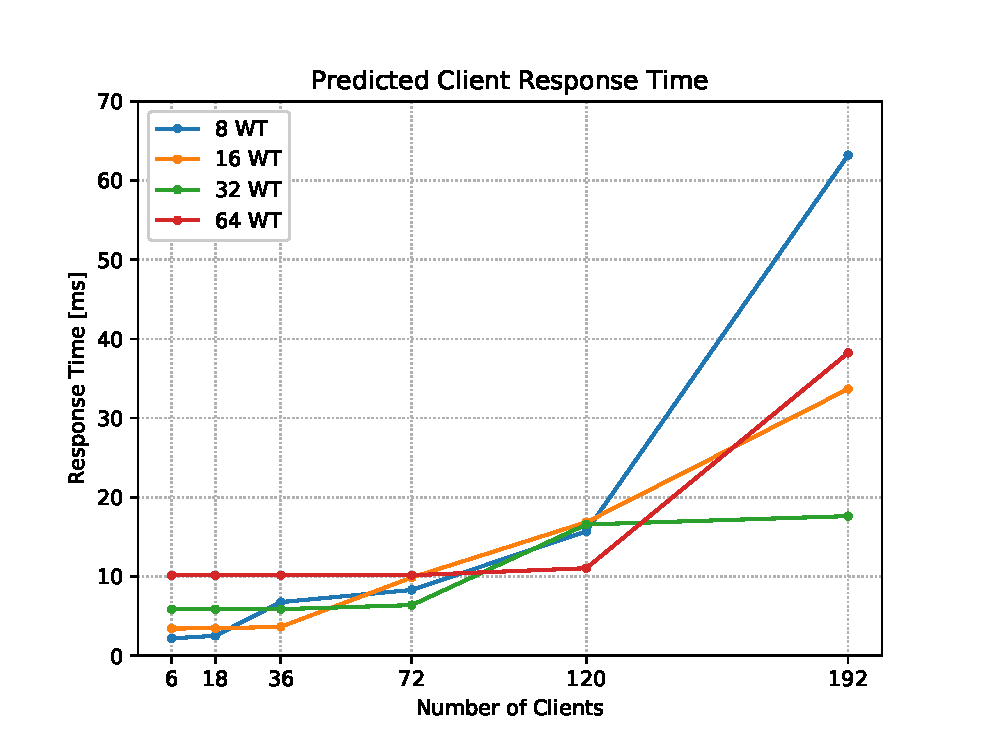
\includegraphics[width=1\linewidth]{plots/7_MMm_ResponseTimePredicted.eps}
    \end{subfigure}
    \begin{subfigure}{.5\textwidth}
        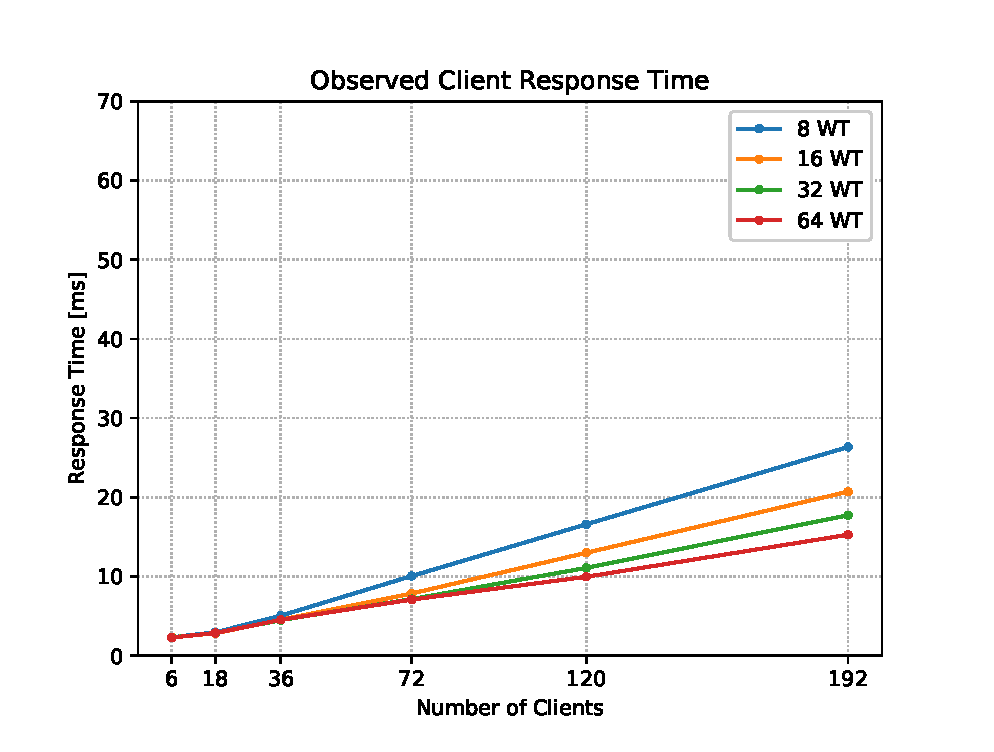
\includegraphics[width=1\linewidth]{plots/7_MMm_ResponseTimeObserved.eps}
    \end{subfigure}
    \caption{M/M/m predicted and measured Response Times, Full System, \autoref{sec7.2}}
    \label{fig:mmm-RT}
\end{figure}

\begin{figure}
    \begin{subfigure}{.5\textwidth}
        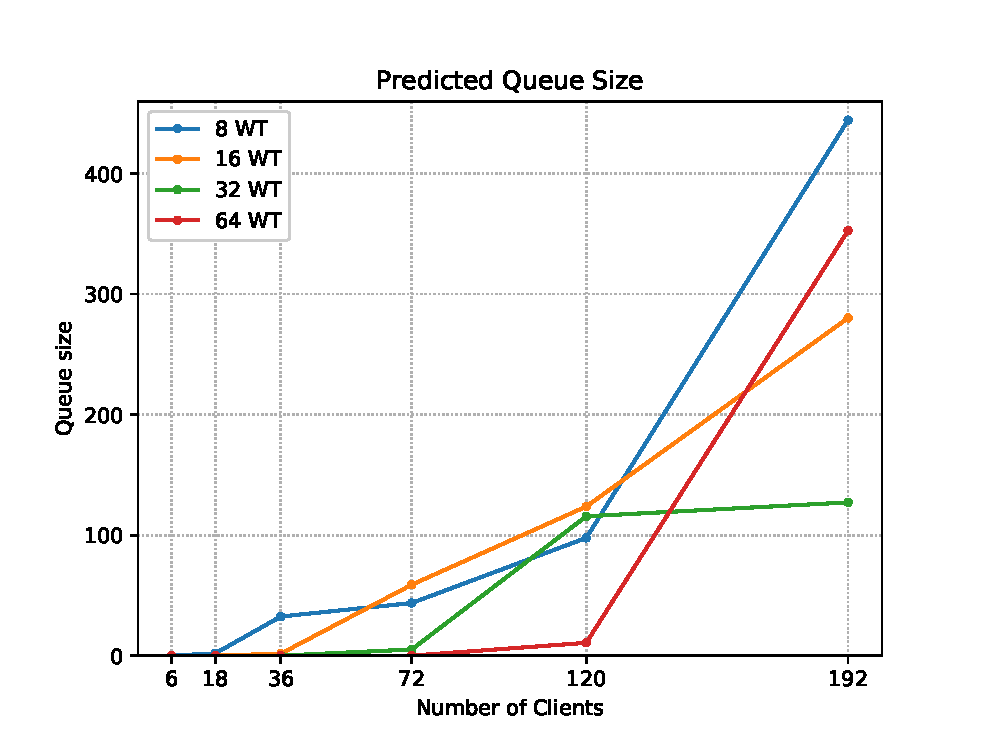
\includegraphics[width=1\linewidth]{plots/7_MMm_QueueSizePred.eps}
    \end{subfigure}
    \begin{subfigure}{.5\textwidth}
        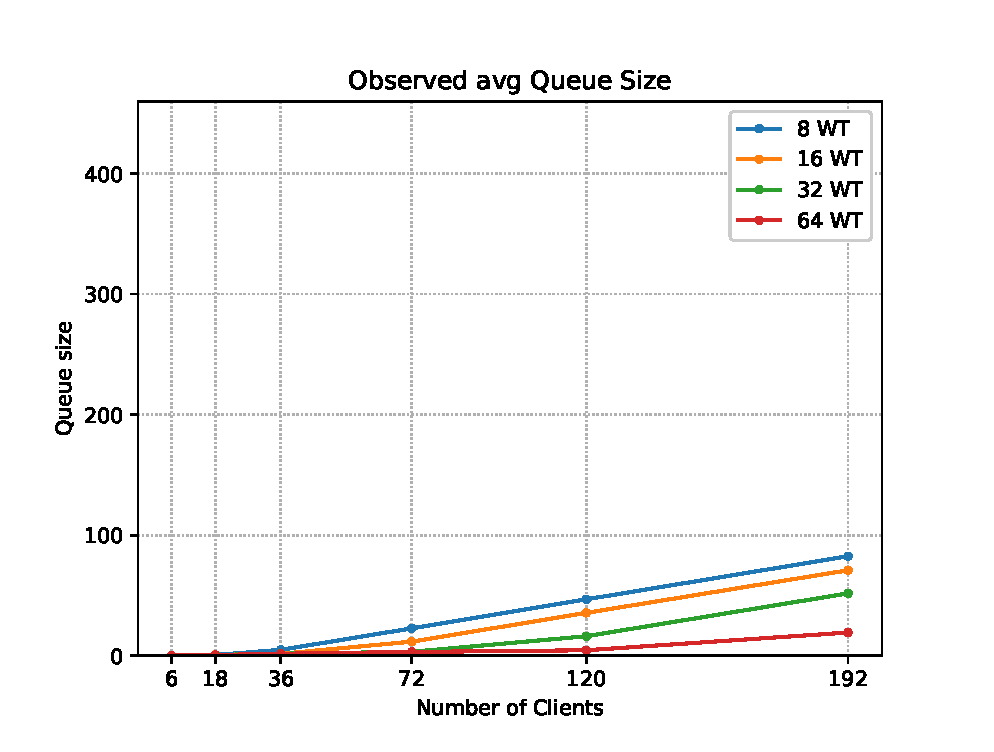
\includegraphics[width=1\linewidth]{plots/7_MMm_QueueSizeObserved.eps}
    \end{subfigure}
    \caption{M/M/m predicted and measured Queue Size, Full System, \autoref{sec7.2}}
    \label{fig:mmm-queueLen}
\end{figure}
\begin{table}
    \begin{subtable}{1.0\linewidth}\centering
        \begin{tabular}{lrrlll}
        \hline
        \# Clients &  $\lambda$ &  $\rho$ &         $E[r]$ &        $E[n\_q]$ &        $E[w]$ \\
        \hline
          6 &    2571.91 &    0.35 &    2.19 // 2.33 &     0.00 // 0.11 &   0.00 // 0.07 \\
         18 &    6093.61 &    0.83 &    2.52 // 2.95 &     1.97 // 0.62 &   0.00 // 0.20 \\
         36 &    7107.66 &    0.97 &    6.77 // 5.06 &    32.53 // 4.87 &   0.00 // 1.87 \\
         72 &    7151.63 &    0.98 &   8.30 // 10.06 &   43.72 // 22.71 &   0.01 // 6.86 \\
        120 &    7229.38 &    0.99 &  15.72 // 16.59 &   97.77 // 46.78 &  0.01 // 13.44 \\
        192 &    7283.78 &    1.00 &  63.21 // 26.35 &  444.42 // 82.55 &  0.06 // 23.17 \\
        \hline
        \end{tabular}
        \caption{8 Worker Threads, $\mu = 7300 / (2*8) = 456 ops/s$}
    \end{subtable}
    \begin{subtable}{1.0\linewidth}\centering
        \begin{tabular}{lrrlll}
        \hline
        \# Clients &  $\lambda$ &  $\rho$ &         $E[r]$ &        $E[n\_q]$ &        $E[w]$ \\
        \hline
          6 &    2577.76 &    0.28 &    3.44 // 2.32 &     0.00 // 0.11 &   0.00 // 0.07 \\
         18 &    6330.40 &    0.68 &    3.45 // 2.84 &     0.06 // 0.70 &   0.00 // 0.12 \\
         36 &    7930.72 &    0.85 &    3.65 // 4.53 &     1.68 // 1.58 &   0.00 // 0.38 \\
         72 &    9159.92 &    0.98 &    9.87 // 7.85 &   58.92 // 11.68 &   0.01 // 3.39 \\
        120 &    9229.22 &    0.99 &  16.85 // 13.00 &  123.78 // 35.57 &   0.01 // 8.55 \\
        192 &    9267.70 &    1.00 &  33.68 // 20.71 &  280.22 // 70.90 &  0.03 // 16.13 \\
        \hline
        \end{tabular}
        \caption{16 Worker Threads, $\mu = 9300 / (2*16) = 291 ops/s$}
    \end{subtable}
    
    \begin{subtable}{1.0\linewidth}\centering
        \begin{tabular}{lrrlll}
        \hline
        \# Clients &  $\lambda$ &  $\rho$ &         $E[r]$ &        $E[n\_q]$ &        $E[w]$ \\
        \hline
          6 &    2596.04 &    0.24 &    5.87 // 2.31 &     0.00 // 0.10 &   0.00 // 0.07 \\
         18 &    6274.84 &    0.58 &    5.87 // 2.86 &     0.00 // 0.66 &   0.00 // 0.12 \\
         36 &    7991.58 &    0.73 &    5.88 // 4.50 &     0.03 // 1.67 &   0.00 // 0.21 \\
         72 &   10070.24 &    0.92 &    6.39 // 7.14 &     5.19 // 3.22 &   0.00 // 0.65 \\
        120 &   10813.54 &    0.99 &  16.57 // 11.09 &  115.68 // 16.18 &   0.01 // 4.09 \\
        192 &   10820.80 &    0.99 &  17.63 // 17.74 &  127.20 // 51.73 &  0.01 // 10.68 \\
        \hline
        \end{tabular}
        \caption{32 Worker Threads, $\mu = 10900 / (2*32) = 170 ops/s$}
    \end{subtable}
    
    \begin{subtable}{1.0\linewidth}\centering
        \begin{tabular}{lrrlll}
        \hline
        \# Clients &  $\lambda$ &  $\rho$ &         $E[r]$ &        $E[n\_q]$ &       $E[w]$ \\
        \hline
          6 &    2611.63 &    0.21 &   10.16 // 2.29 &     0.00 // 0.10 &  0.00 // 0.07 \\
         18 &    6262.69 &    0.50 &   10.16 // 2.87 &     0.00 // 0.60 &  0.00 // 0.12 \\
         36 &    7933.14 &    0.63 &   10.16 // 4.53 &     0.00 // 1.62 &  0.00 // 0.21 \\
         72 &   10147.69 &    0.81 &   10.16 // 7.09 &     0.05 // 3.13 &  0.00 // 0.34 \\
        120 &   12036.31 &    0.96 &   11.05 // 9.96 &    10.71 // 4.52 &  0.00 // 0.46 \\
        192 &   12565.70 &    1.00 &  38.23 // 15.27 &  352.76 // 19.24 &  0.03 // 3.93 \\
        \hline
        \end{tabular}
        \caption{64 Worker Threads, $\mu = 12600 / (2*64) = 98 ops/s$}
    \end{subtable}

    \caption{System Properties, M/M/m Model. Please note that in the three rightmost columns the values are displayed as $predicted  //  observed$. $E[r]$ is the response time in ms,  $E[n\_q]$ displays the number of requests in the queue and $E[w]$ displays is the queue waiting time in ms.  }
    \label{MMm}
\end{table}

\subsection{Network of Queues} \label{sec7.3}



%Based on Section 3, build a network of queues which simulates your system. Motivate the design of your network of queues and relate it wherever possible to a component of your system. Motivate your choice of input parameters for the different queues inside the network. Perform a detailed analysis of the utilization of each component and clearly state what the bottleneck of your system is. Explain for which experiments the predictions of the model match and for which they do not.
% Q: For Section 7, which exact configuration should I use for network of queues?
% A: You need to consider both 1 and 2 middleware configuration. You need to analyze both read only and write only workloads. You can set the number of worker threads to the constant that delivers highest throughput.

\begin{figure}
    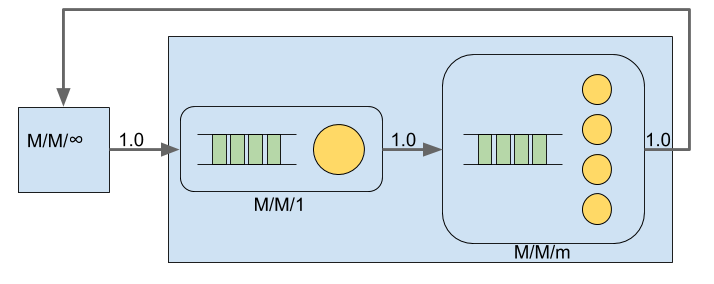
\includegraphics[width=.7\linewidth]{plots/NetworkOfQueues1MW.png}
    \caption{Network of Queues for 1 Middleware}
    \label{fig:7-3:1MW}
\end{figure}

\begin{figure}
    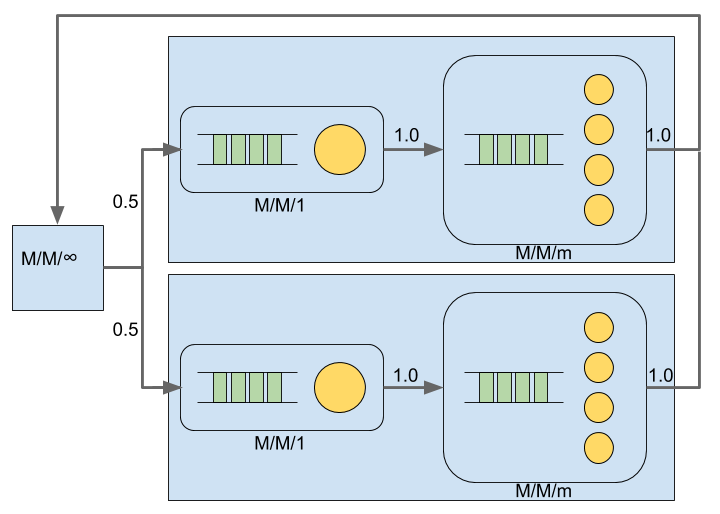
\includegraphics[width=.7\linewidth]{plots/NetworkOfQueues2MW.png}
    \caption{Network of Queues for 1 Middleware}
    \label{fig:7-3:2MW}
\end{figure}

\end{document}
